%!TEX root=masterproef.tex

\chapter{Achtergrond}
\label{chapter:achtergrond}

In het inleidende hoofdstuk werd het concept DSN al kort ge\"introduceerd. In
dit hoofdstuk wordt het kader geschetst waarbinnen we op zoek gaan naar
antwoorden.

Sectie \ref{section:landscape} brengt het landschap van draadloze
sensornetwerken in kaart: wat typeert en onderscheidt hen van andere netwerken?
Wie is de aanvaller en wat zijn zijn doelen? Waarom is het vaststellen van
inbraken een belangrijk onderzoeksdomein?

Sectie \ref{section:related} gaat in op gerelateerd onderzoek. Een doelstelling
van deze masterproef is ook het in kaart brengen van de mogelijkheden en
beperkingen betreffende al beschreven methodes om inbraken vast te stellen.

Bij de beschrijving van de verschillende oplossingen zal tevens kritisch
nagegaan worden in hoeverre deze in een realistische situatie effectief
bijdragen tot het detecteren van inbreuken in het netwerk.

%!TEX root=masterproef.tex

\section{Draadloze sensornetwerken}
\label{section:landscape}

``\emph{Waarom is het belangrijk om beveiliging van draadloze sensornetwerken
te bestuderen? Dit is toch al uitvoerig gedaan voor andere vormen van
netwerken!?}'' Op het eerste zicht is dit een zeer valabele opmerking. Reeds
sinds de late jaren '80 kennen we concepten als \emph{firewalls}, virussen,
wormen\dots Meer dan 30 jaar reeds wordt er onderzoek gedaan naar
computerbeveiliging en solide oplossingen zijn bedacht, uitgewerkt en
ge\"implementeerd. Wat houdt ons tegen om deze toe te passen op draadloze
sensornetwerken?

\subsection{Eigenschappen}

Ondanks het feit dat knopen in essentie kleine computers zijn en de
verbindingen die tussen hen tot stand komen een netwerk worden genoemd, eindigt
daar de vergelijking volledig. Draadloze sensoren en hun netwerken zijn een
wereld op zich, met zeer typerende eigenschappen, regels, mogelijkheden en
beperkingen.

Een draadloze sensor is inderdaad een kleine computer, maar de nadruk ligt hier
op \emph{kleine}. De rekenkracht van een knoop is slechts een fractie van deze
van een hedendaagse computer en ligt in de tientallen megahertz (MHz) - waar we
bij hedendaagse systemen spreken in termen van gigahertz (GHz). De reden is
evident: draadloze sensornetwerken zijn draadloos en worden ingezet in de meest
uiteenlopende en afgelegen situaties. Ze zijn daarom gedurende lange tijd
afhankelijk van een zelfde batterijvoeding, die dan ook optimaal benut moet
worden.

Ook het netwerk dat ze vormen vertoont typische eigenschappen die sterk
verschillen van de meer klassieke computernetwerken. Zo identificeert
\citep{blilat2012wireless} zes unieke eigenschappen van een DSN:

\begin{description}

  \item[Boomstructuur] De routering van de meeste draadloze sensornetwerken is
  \emph{gestructureerd als een boom}. De concepten co\"ordinator (of
  basisstation), router en eindknoop werden eerder, samen met hun structuur,
  ge\"identificeerd in sectie \ref{subsection:topologie}.

  \item[Aggregatie en redundantie] De gegevens door een knoop uit het netwerk
  verzameld, worden typisch niet op zich beschouwd, maar \emph{geaggregeerd}
  met deze van andere knopen. Dit wordt enerzijds gedaan om te compenseren voor
  effectieve aberraties in de metingen zelf, maar ook om de onzekerheid van de
  beschikbaarheid van knopen te ondervangen.

  \item[Vervangbaar] Knopen zijn typisch de goedkopere onderdelen van het
  netwerk en ze staan slechts ten dienst van het eigenlijke doel van het
  netwerk, het verzamelen van gegevens. Om die reden zijn ze eenvoudig
  vervangbaar en dit wordt als een inherente eigenschap gezien. Het netwerk
  \emph{tolereert storingen} ten gevolge van het wegvallen van knopen en vangt
  ze op door redundantie en aggregatie.

  \item[Verwerking in het netwerk] Om er voor te zorgen dat het netwerk zo min
  mogelijk belast wordt met het verzenden van gegevens, worden meetgegevens zo
  dicht mogelijk bij de oorspronkelijke knoop \emph{gefilterd en verwerkt}.

  \item[Uniformiteit] Een draadloos sensornetwerk bestaat uit knopen en niets
  anders. Elke knoop kan tegelijkertijd \emph{sensor} of \emph{router} zijn,
  wat resulteert, in combinatie met de voorgaande eigenschappen, in een
  reductie van het netwerkverkeer.

  \item[Energiebesparing] De werking van een knoop kent een typisch
  \emph{gefaseerd zendpatroon}: het verzamelen van meetgegevens, het ontvangen
  van gegevens van andere knopen en het doorsturen van geaggregeerde gegevens
  naar hogerliggende knopen. Hierdoor kan elke knoop zijn radio gedurende
  bepaalde periodes volledig afzetten om energie te besparen.

\end{description}

Dit beeld vinden we ook terug bij \citep{aschenbruck2012security} die de
situatie van draadloze sensornetwerken samenvat in drie zeer typische en
problematische bronnen van beveiligingsproblemen: 

\begin{itemize}[noitemsep, topsep=0pt, partopsep=0pt]

  \item{Beperkingen qua middelen en dan vooral de energievoorziening.}
  
  \item{Fysieke toegankelijkheid die leidt tot de mogelijkheid om knopen te
  veroveren.}

  \item{Verwerking van gegevens die reeds binnen het netwerk gebeurt, waardoor
  het bv. onmogelijk wordt om encryptie toe te passen tussen zender en
  ontvanger, waardoor tussenliggende verwerking eigenlijk uitgesloten wordt.}

\end{itemize}

\subsection{Inbraakdetectie}

\citep{zhang2000intrusion} geeft een zeer algemene, maar zeer correcte
definitie van inbraakdetectie:

\begin{quote}
\emph{Intrusion detection ... involves capturing audit data and reasoning about
the evidence in the data to determine whether the system is under attack.}
\end{quote}

Inbraakbeveiliging omvat twee essenti\"ele activiteiten: het vastleggen van
auditgegevens en het redeneren over deze gegevens. In het geval van draadloze
sensornetwerken moeten we het aspect \emph{systeem} op twee manieren
interpreteren: enerzijds als een knoop en anderzijds als het hele netwerk op
zich. Dit onderscheid bestaat ook in meer klassieke computernetwerken in de
vorm van inbraakdetectie voor \emph{systemen} en \emph{netwerken}.

In de context van draadloze sensornetwerken zal dit onderscheid zich echter
veel meer profileren omdat het netwerk hier geen centraal medium is. Daar waar
het netwerk in een klassieke opstelling typisch vanuit \'e\'en systeem kan
gecontroleerd worden door het afleiden van alle netwerkverkeer naar \'e\'en
enkele detectiemodule, is dit in het geval van een DSN niet mogelijk. Het
draadloze aspect maakt dat er geen controleerbare toegangswegen zijn naar elke
knoop en dat dus elke knoop letterlijk op zichzelf aangewezen is.

Samen met het wegvallen van een centrale inbraakdetectie, valt ook de centrale
bescherming op netwerkniveau weg. Binnen een DSN is het ook niet mogelijk om te
genieten van de bescherming van een \emph{firewall}. Er is geen alles omarmende
bescherming, niet op logisch of netwerkvlak, maar ook niet op fysiek vlak.
Aangezien draadloze sensornetwerken typisch open en bloot in de buitenwereld
ge\"installeerd worden, en dit voor langere periodes zonder aanwezigheid van
een eigenaar, kunnen ze ook fysiek benaderd worden door ieder die dat wil.
Zelfs de elementaire zekerheid van een fysieke bescherming bv. in een
datacenter, komt bij draadloze sensornetwerken volledig te vervallen.

Terecht stelt \citep{perrig2004security} daarom ook dat de eerste zorg omtrent
de beveiliging van draadloze sensornetwerken een veilige manier om de groep van
sensoren te beheren moet zijn. De manier waarop nieuwe knopen in het netwerk
worden opgenomen en de beveiliging van de onderlinge communicatie, is van
primordiaal belang. Voorkomen is beter dan genezen.

Maar we moeten ook realistisch zijn. Geen door mensenhanden gemaakt systeem is
feilloos en nagenoeg elk ge\"informatiseerd systeem zal met de nodige inzet en
moeite veroverd kunnen worden. Op dat ogenblik is het belangrijk dat er een
tweede verdedigingslinie is: inbraakdetectie. In het geval van DSN is dit
misschien nog meer prangend, omdat er niet langer een fysieke bescherming, noch
een centrale netwerkbescherming in de vorm van bv. een \emph{firewall} is.

\subsection{De tegenstander en zijn aanvallen}

Tijd om kennis te maken met de tegenstander. Wat is zijn doel? Welke middelen
heeft hij ter beschikking? Hoe kunnen we zijn aanvallen identificeren?

Identificatie van aanvallen wordt door \citep{zhang2000intrusion} gecatalogeerd
als \emph{misbruik} of \emph{anomalie}. Misbruik kan typisch gedetecteerd
worden aan de hand van patronen, terwijl voor het detecteren van anomalie\"en
er een patroon moet opgesteld worden en aberraties van dat patroon vastgesteld.
Vooral dit laatste is een delicaat aspect. Zo is het niet eenvoudig om
onderscheid te maken tussen een knoop die verplaatst werd, en tijdelijk
verkeerde routing informatie verspreid, en een knoop die veroverd werd en
kwaadwillig foutieve informatie uitstuurt.

\citep{aschenbruck2012security} identificeert vier fundamentele doelen die
nagestreefd worden door een aanvaller: (1) het manipuleren van gegevens, (2)
het afluisteren van communicatie, (3) het tegenhouden van gegevens en (4)
toegang verkrijgen tot het netwerk. Figuur \ref{fig:wsn-threat-analysis} geeft
een schematisch overzicht van deze dreigingsanalyse.

\begin{figure}[ht]
  \centering
  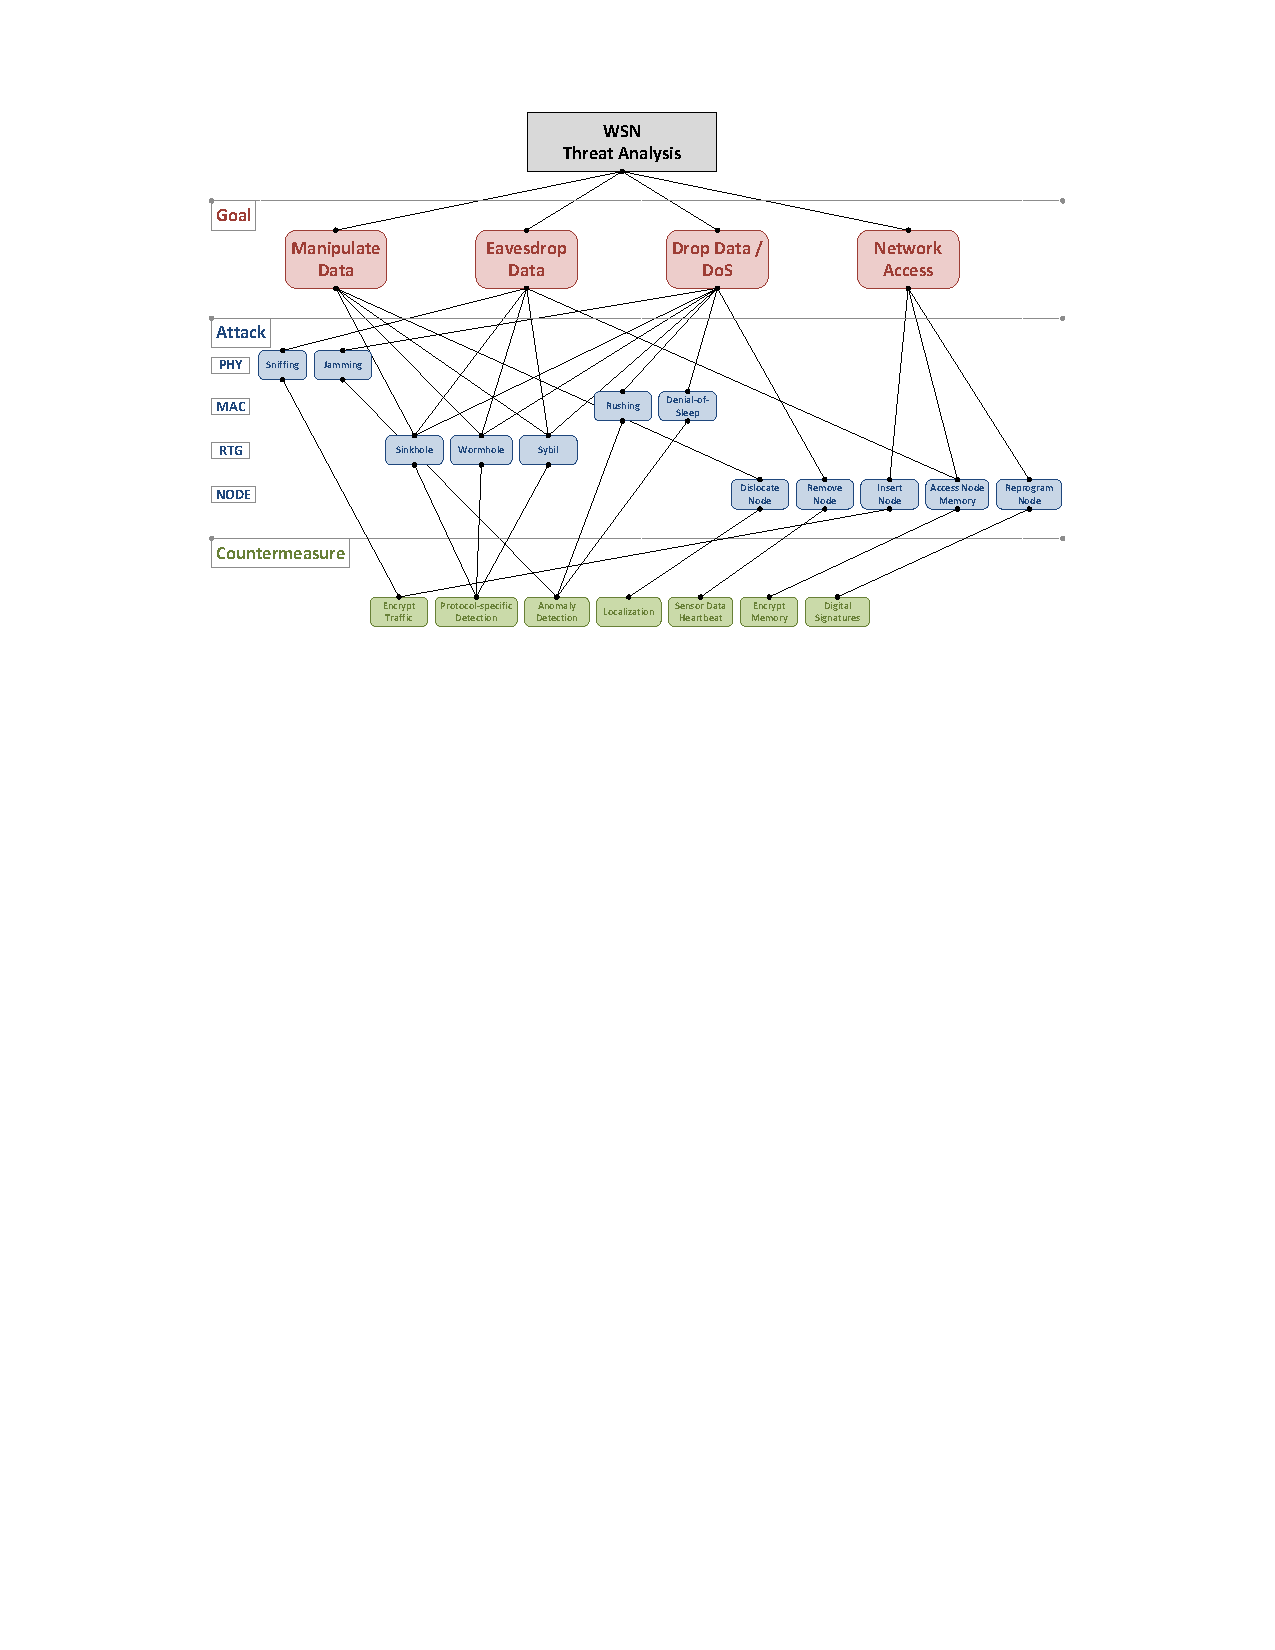
\includegraphics[width=0.95\linewidth]{resources/wsn-threat-analysis.pdf}
  \caption[Dreigingsanalyse van een DSN]{Dreigingsanalyse van een DSN (Bron:\citep{aschenbruck2012security})}
  \label{fig:wsn-threat-analysis}
\end{figure}

\vspace{-5mm}

\subsubsection*{Applicatie laag}

Een niveau dat hier nogal nadrukkelijk ontbreekt is dat van de applicatie.
Bovenop de verschillende netwerklagen van een sensorknoop, zal de sensor nog
typisch een niveau kennen dat specifiek is voor het desbetreffende DSN. Het
bevat de functionaliteit die het netwerk zijn bestaansreden geeft.

Ondanks de overvloed aan mogelijke aanvallen op de standaard netwerklagen, mag
het bestaan van de applicatielaag niet uit het oog verloren worden. Het
merendeel van aanvallen spitst zich net toe op fouten in deze laag. Deze kunnen
tevens dikwijls uitgebuit worden met normale vormen van communicatie. Zo hoeft
een aanvaller geen aanvallen op te zetten zoals de hoger vermelde voorbeelden,
als hij eenvoudig een legitieme boodschap kan zenden naar een gewone knoop en
een antwoord kan ontvangen met de informatie die hij wenst.

Op deze manier is er ook geen sprake van ``te detecteren malafide gedrag'' en
zal de aanval dikwijls onopgemerkt gebeuren. We denken hier aan klassieke
aanvallen zoals bv. \emph{buffer overflows}, waarbij andere gegevens uit het
geheugen worden gelezen dan bedoeld.

%!TEX root=masterproef.tex
\section{Gerelateerd onderzoek}
\label{section:related}

Het detecteren van inbraken komt dikwijls neer op het detecteren van abnormaal
gedrag of algemeen anomalie\"en. Er zijn tal van manieren hoe normaal gedrag
kan gedefinieerd worden elk met hun voor- en nadelen, beperkingen en successen.
(\ref{subsection:anomaly}).

Met de komst van draadloze sensornetwerken moesten veel klassieke
beveiligingstechnieken volledig herbekeken worden. De schaal waarop deze
netwerken opereren, maar vooral de fysieke toegankelijkheid waren parameters
die niet als problemen beschouwd ervaren werden in meer klassieke computer
netwerken. Hierdoor moesten fundamentele eigenschappen die niet langer
eenvoudig technologisch konden afgedekt worden, opnieuw gedefinieerd worden. Zo
leidt de hoge graad van distributie en de beperkte mogelijkheden tot onderlinge
communicatie tot een basisgegeven van reputatie en vertrouwen
(\ref{subsection:reputation}).

Anderzijds zal snel blijken dat een enkele knoop niet eenvoudig kan beslissen
of hij al dan niet een andere knoop vertrouwd. Knopen zullen - en dit is
eigenlijk een fundamentele eigenschap van draadloze sensornetwerk - moeten
samenwerken. De nood voor co\"operatieve algoritmen
(\ref{subsection:cooperation}) is hier een belangrijke volgende bouwsteen.

Maar hoe voeden we dit co\"operatief opgebouwd vertrouwen in een omgeving waar
een aanvaller fysieke toegang heeft tot elke knoop en zowel de vluchtige als de
programma geheugens kan benaderen en wijzigen? Een logische piste is om op zoek
te gaan naar een manier om de programma code die op een knoop ge\"installeerd
is te valideren voor dat deze aangeroepen en vertrouwd wordt. Is het derhalve
mogelijk om software attestatie (\ref{subsection:attestation}) te doen?
Eigenlijk is software attestatie slechts een specifieke vorm van het nagaan van
de integriteit van een bepaald aspect van een knoop. In dit geval gaat het om
de inhoud van het geheugen. In het algemeen kan dit beschouwd worden als het
opsporen van anomalie\"en.

Naast detectiealgoritmen zijn er ook reeds pogingen gedaan om alles omvattende
raamwerken te cre\"eren die het detecteren en verijdelen van aanvallen
makkelijker moeten maken. (\ref{subsection:frameworks}).

Enkele werken die zelf een goed overzicht bieden van de stand van zake met
betrekking tot inbraakdetectie in DSN zijn o.a. \citep{mishra2004intrusion} end
\citep{alrajeh2013intrusion}. Naast grote overlappingen met de hierna
gepresenteerde topics, bevatten ze nog andere voorbeelden en/of indelingen
omtrent deze materie.

%!TEX root=masterproef.tex

\subsection{Detecteren van anomalie\"en}
\label{subsection:anomaly}

Een anomalie is een afwijking van een normaal verloop van gebeurtenissen of
iets of iemands gedrag. Een knoop uit een DSN heeft een redelijk eenvoudig en
constante levensloop. Typisch zal een knoop op regelmatige tijdstippen
\emph{wakker worden}, waarden opmeten aan de hand van zijn sensoren en deze
waarden doorsturen naar een centrale locatie. Verder zal een knoop, als
onderdeel van het netwerk, tevens zulke waarden van andere knopen doorsturen.
Dit patroonmatige gedrag kan ge\"identificeerd worden en in een model verwerkt
worden. Op basis van zulk een model kan vervolgens nagegaan worden of de acties
van een knoop op een gegeven moment in lijn zijn met het model of dat er sprake
is van een anomalie.

Zulk een afwijking van het verwachte gedrag kan wijzen op veranderingen van
buitenaf. Deze kunnen op hun beurt veroorzaakt zijn door een aanval op het
netwerk. Aangezien we niet alle communicatie van en naar knopen kunnen
onderscheppen en eventuele aanvallen kunnen detecteren, kunnen
anomaliegebaseerde dectectiemechanismen helpen om op basis van neveneffecten
toch aanvallen te detecteren, of althans toch de gevolgen ervan.

\subsubsection*{Anomali\"en, afwijkingen, aberraties}
\label{subsubsection:outlier}

\citep{zhang2010outlier} is een excellent overzicht van methoden om anomali\"en,
afwijkingen of aberraties (\emph{outliers}) te detecteren in een reeks
van metingen. Het belicht enerzijds de fundamentele technieken die ter
beschikking staan om deze aberraties op te merken maar tracht ook een
classificatie en taxonomie op te stellen hiervoor.

De auteurs stellen dat het detecteren van afwijkingen behoort tot het domein
van \emph{datamining} en dat het in die context reeds uitvoerig onderzocht is,
evenals binnen disciplines as statistiek, machinaal leren, informatie
theorie \dots. Aangezien het kunnen uitsluiten van afwijkingen de verwerking
van de overblijvende meetresultaten sterk positief be\"invloed is het in het
kader van DSN uitermate interessant.

Toch kan eerder onderzoek opnieuw niet eenvoudig toegepast worden in het kader
van DSN. De beperkte middelen van de sensorknoop schrappen al veel van de
klassieke oplossingen die bv. gecentraliseerd werken. De overdaad aan
communicatie die nodig is om voldoende gegevens te centraliseren voor
verwerking is niet realistisch in het kader van een DSN. Ook zijn veel van de
algoritmen typisch niet ontwikkeld met de beperkte rekenmogelijkheden van
sensorknopen. De conclusie is dat er een balans moet gevonden worden tussen de
mogelijkheden van datamining algoritmen voor het detecteren van afwijkingen en
de verhouding van hun noden ten opzichte van de middelen van de knopen.

\subsubsection*{Neurale netwerken}
\label{subsubsection:neuralnetworks}

Wanneer men denkt aan het vastleggen van een patroon en het controleren of een
bepaalde situatie voldoet aan dat patroon wordt in informatiecakringen ook snel
verwezen naar neurale netwerken. Neurale netwerken kunnen immers
\emph{getraind} worden door middel van een aantal goede (en slechte)
voorbeelden, waarna nieuwe voorbeelden kunnen gecatalogeerd worden als ook goed
of slecht. De complexiteit van het bepalen van deze beslissing is typisch
redelijk eenvoudig en lijkt zich daarom uitermate goed te lenen voor het
detecteren van anomalie\"en door sensorknopen.

In \citep{ramesh2012wireless} volgen de auteurs deze denkpiste, maar stellen
tevens dat er betere methoden bestaan. Ze trachten twee specifieke aanvallen
het hoofd te bieden: DoS en passieve informatie vergaring en vergelijken
hierbij een aanpak op basis van een neuraal netwerk en hun eigen aanpak op
basis van encryptie op basis van symmetrische sleutels.

Ofschoon dat sommige van hun veronderstelling na\"ief zijn (zo baseren ze zich
op een gedeelde geheime sleutel van 8 bits), toont hun werk wel aan dat een
aanpak met neurale netwerken eenvoudig te realiseren is en een valabele piste
kan zijn om anomaliedetectie te doen.

\subsubsection*{Voorspellingen}
\label{subsubsection:predictions}

Waar neurale netwerken in staat zijn om op basis van voorbeelden een nieuwe
situatie te catalogeren, kan men aan de hand van een Markov model
voorspellingen doen over de toekomst.

Het is deze piste dat onderzocht wordt in \citep{zhijie2012intrusion}. Opnieuw
betreft het een poging om DoS aanvallen te detecteren. De bedoeling is dat
sensorknopen individueel bepalen of er een DoS aanval bezig is. Volgens de
auteurs is dit mogelijk aan de hand van een Markov model dat het netwerkverkeer
voorspelt.

Het model wordt zo geconstrueerd dat er een verband ontstaat tussen de toestand
van een knoop in relatie tot het tijdstip en de verwachtte hoeveelheid gegevens
die verstuurd zouden kunnen worden.

Het idee achter het artikel lijkt een mogelijke piste, maar omtrent veel
belangrijke details blijven echter zeer vaag, waardoor de volledige toedracht
van het algoritme niet eenduidig ingeschat kan worden. Zo wordt bv. nauwelijks
ingegaan op wat de toestand van een knoop juist bepaalt of hoe de
hoeveelheid gegevens die verstuurd kunnen worden wanneer een knoop zich in een
bepaalde toestand bevindt, bepaald wordt.

%!TEX root=masterproef.tex

\subsection{Reputatie en vertrouwen}
\label{subsection:reputation}

De probleemstelling dat knopen in het netwerk elkaar niet langer kunnen
vertrouwen, zette verschillende onderzoekers aan tot het zoeken naar
oplossingen gebaseerd op reputatie en vertrouwen.

\citep{ganeriwal2008reputation} beschrijft een architectuur gebaseerd op
observaties door knopen van de acties van andere knopen in het kader van acties
van zichzelf of derde knopen. Figuur \ref{fig:reputation-cooperation} toont de
situaties die beschouwd worden: in \ref{fig:reputation-cooperative-node} zal
een co\"operatieve knoop (C) alle boodschappen die via hem verzonden worden
door een zendende knoop (Z) effectief doorsturen naar een verdergelegen
ontvangende knoop (O). De verzender van de boodschap, alsook andere naburige
knopen (B) kunnen deze actie vaststellen. In
\ref{fig:reputation-uncooperative-node} daarentegen zal een een
niet-co\"operatieve knoop (NC) deze boodschappen niet verder versturen of zelfs
aanpassen.

\begin{figure}
\centering
\begin{subfigure}{.49\textwidth}
\centering
  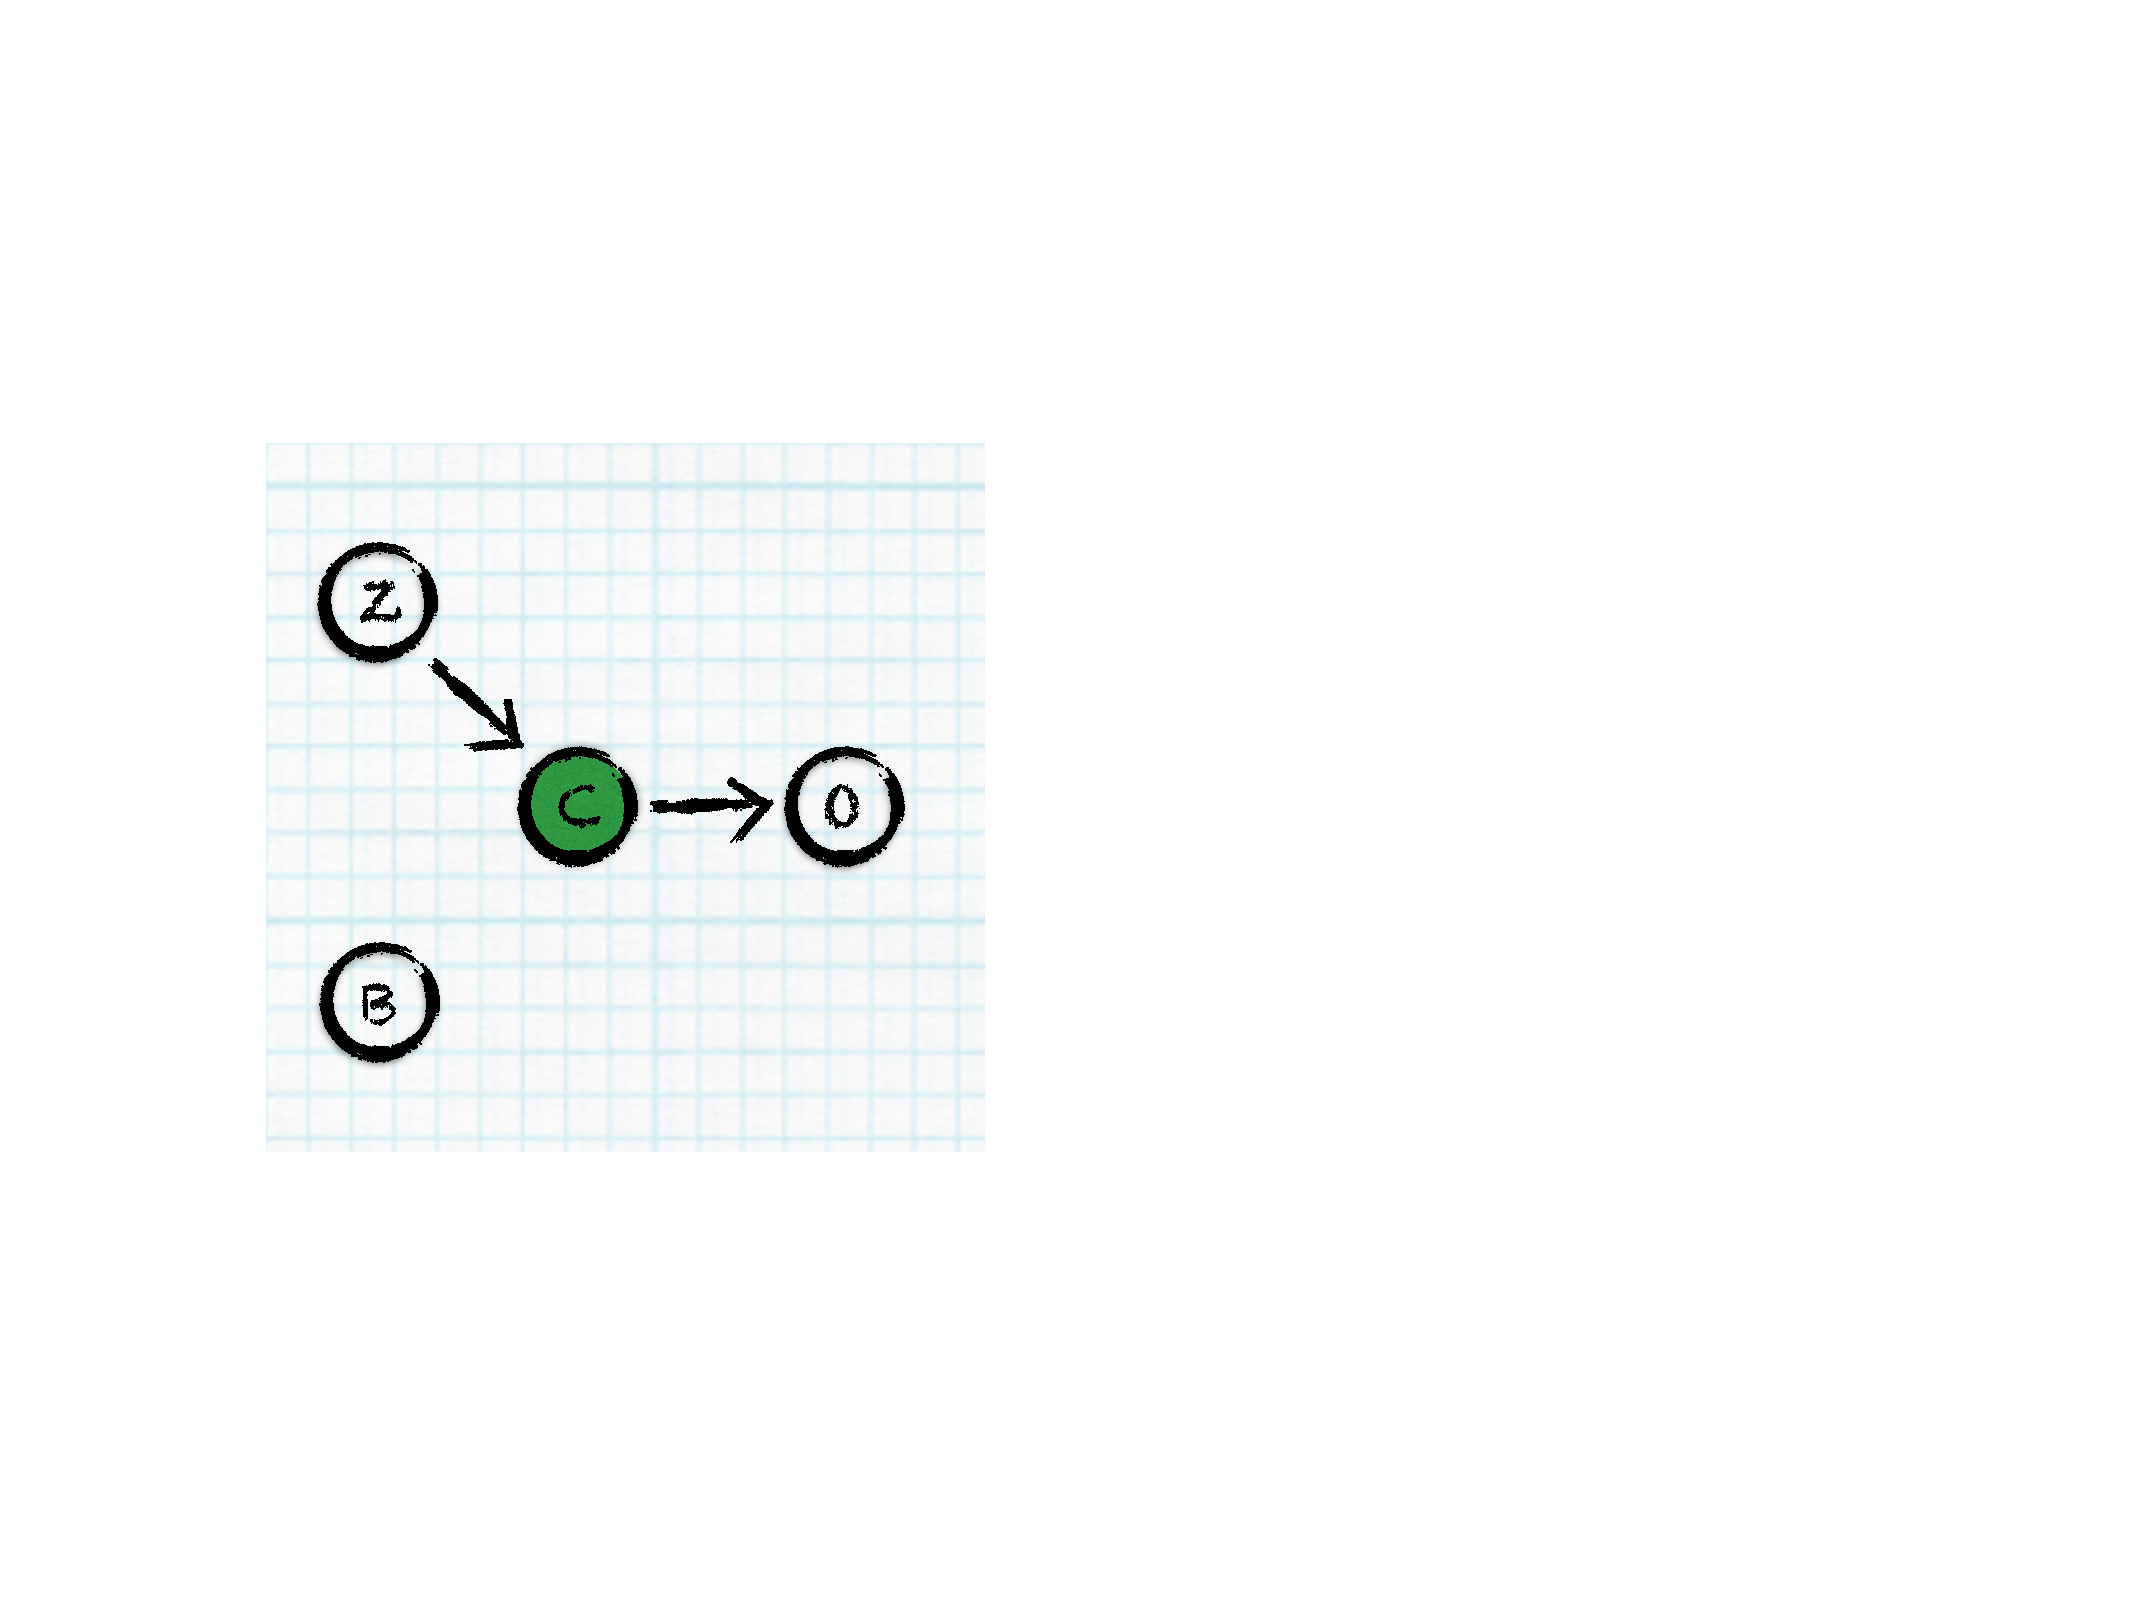
\includegraphics[width=.8\linewidth]{./resources/cooperative.pdf}
  \caption{Co\"operatieve knoop}
  \label{fig:reputation-cooperative-node}
\end{subfigure}
\begin{subfigure}{.49\textwidth}
\centering
  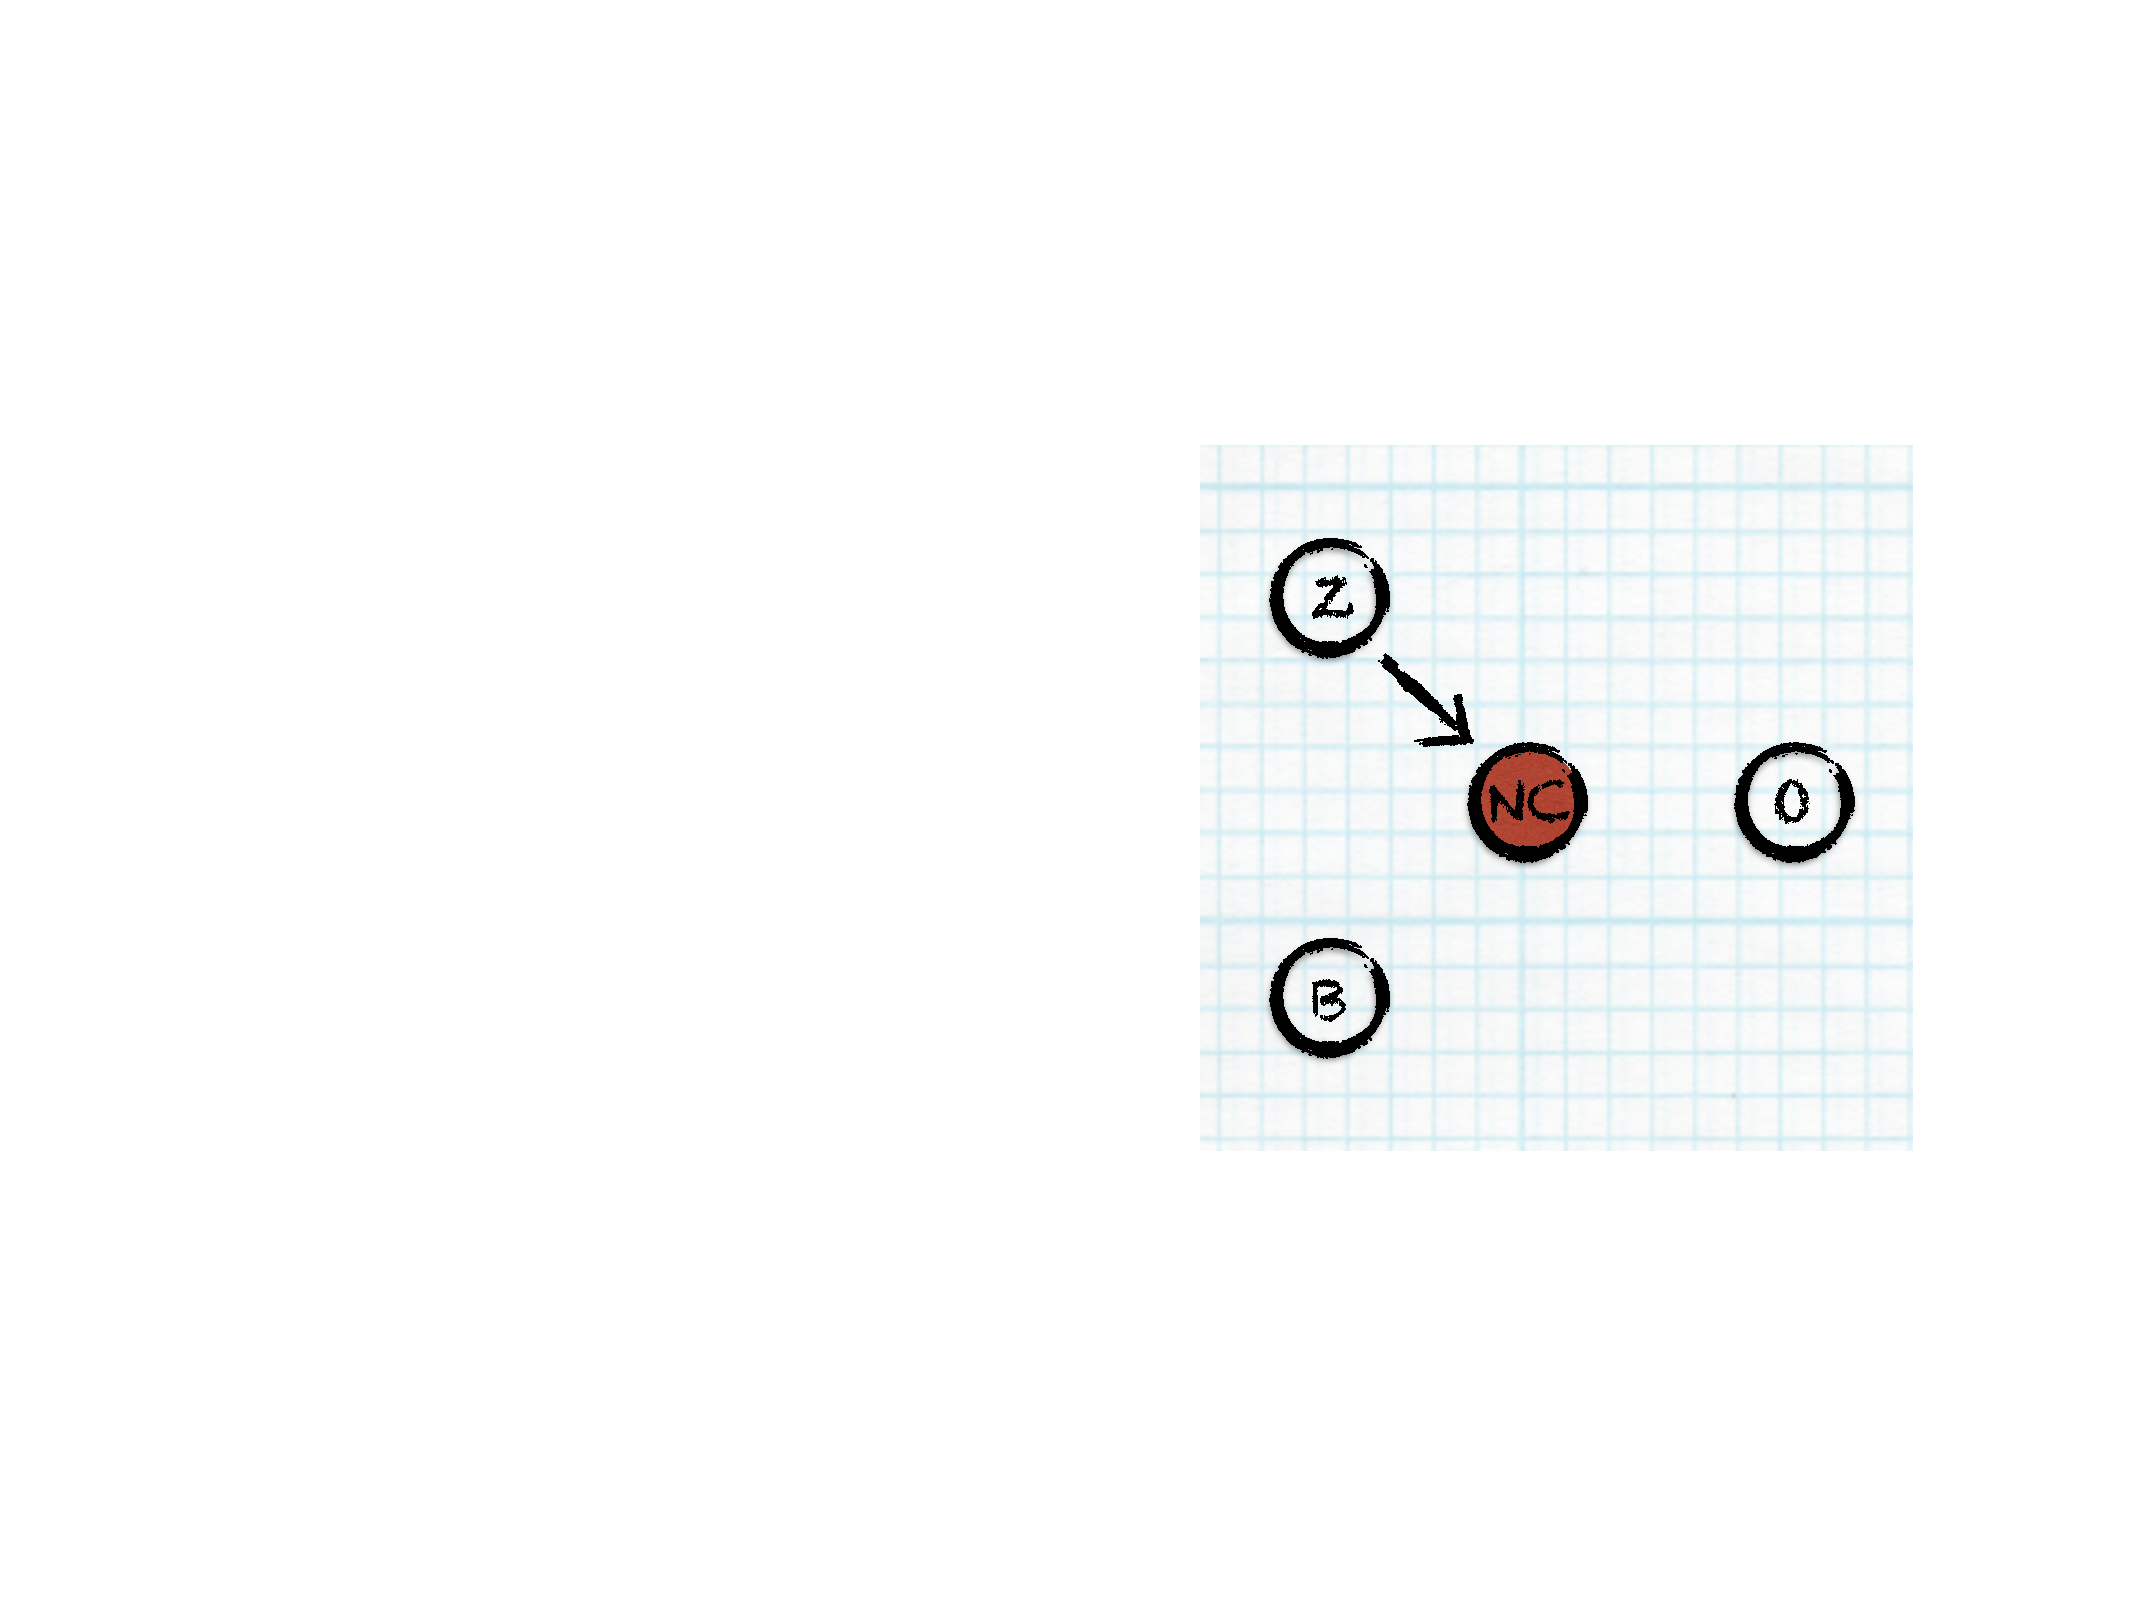
\includegraphics[width=.8\linewidth]{./resources/non-cooperative.pdf}
  \caption{Niet-co\"operatieve knoop}
  \label{fig:reputation-uncooperative-node}
\end{subfigure}
\caption{Beschouwde situaties bij al dan niet co\"operatieve knopen}
\label{fig:reputation-cooperation}
\end{figure}

Op basis van deze situatie stellen de auteurs dat de reputatie van een knoop
kan weergegeven worden aan de hand van een beta distributie. Bijlage
\ref{appendix:reputation} bespreekt de mathematische onderbouw hiervan.

De auteurs vermelden zelf een zeer belangrijk probleem: omdat knopen constant
moeten luisteren naar de acties van naburige knopen, moeten zij constant actief
zijn. Dit is een zeer nadelig uitgangspunt voor systemen die typisch trachten
zuinig om te springen met hun energie.

Maar de architectuur heeft ook inherente problemen en laat kwaadwillige
partijen toe om - mits kennis van de parameters - net onder de radar te
opereren. We illustreren dit met de simulatie zoals deze uitgevoerd werd door
de auteurs.

De evolutie van een volledige co\"operatieve of volledige niet-co\"operatieve
knoop wordt weergegeven in figuur \ref{fig:reputation-paper}. Een eigenschap
van het algoritme is dat pas na een tiental (louter positieve) observaties een
knoop de drempelwaarde van vertrouwen overschrijdt.

\begin{figure}[ht]
\centering
\begin{subfigure}{.49\textwidth}
  \centering
  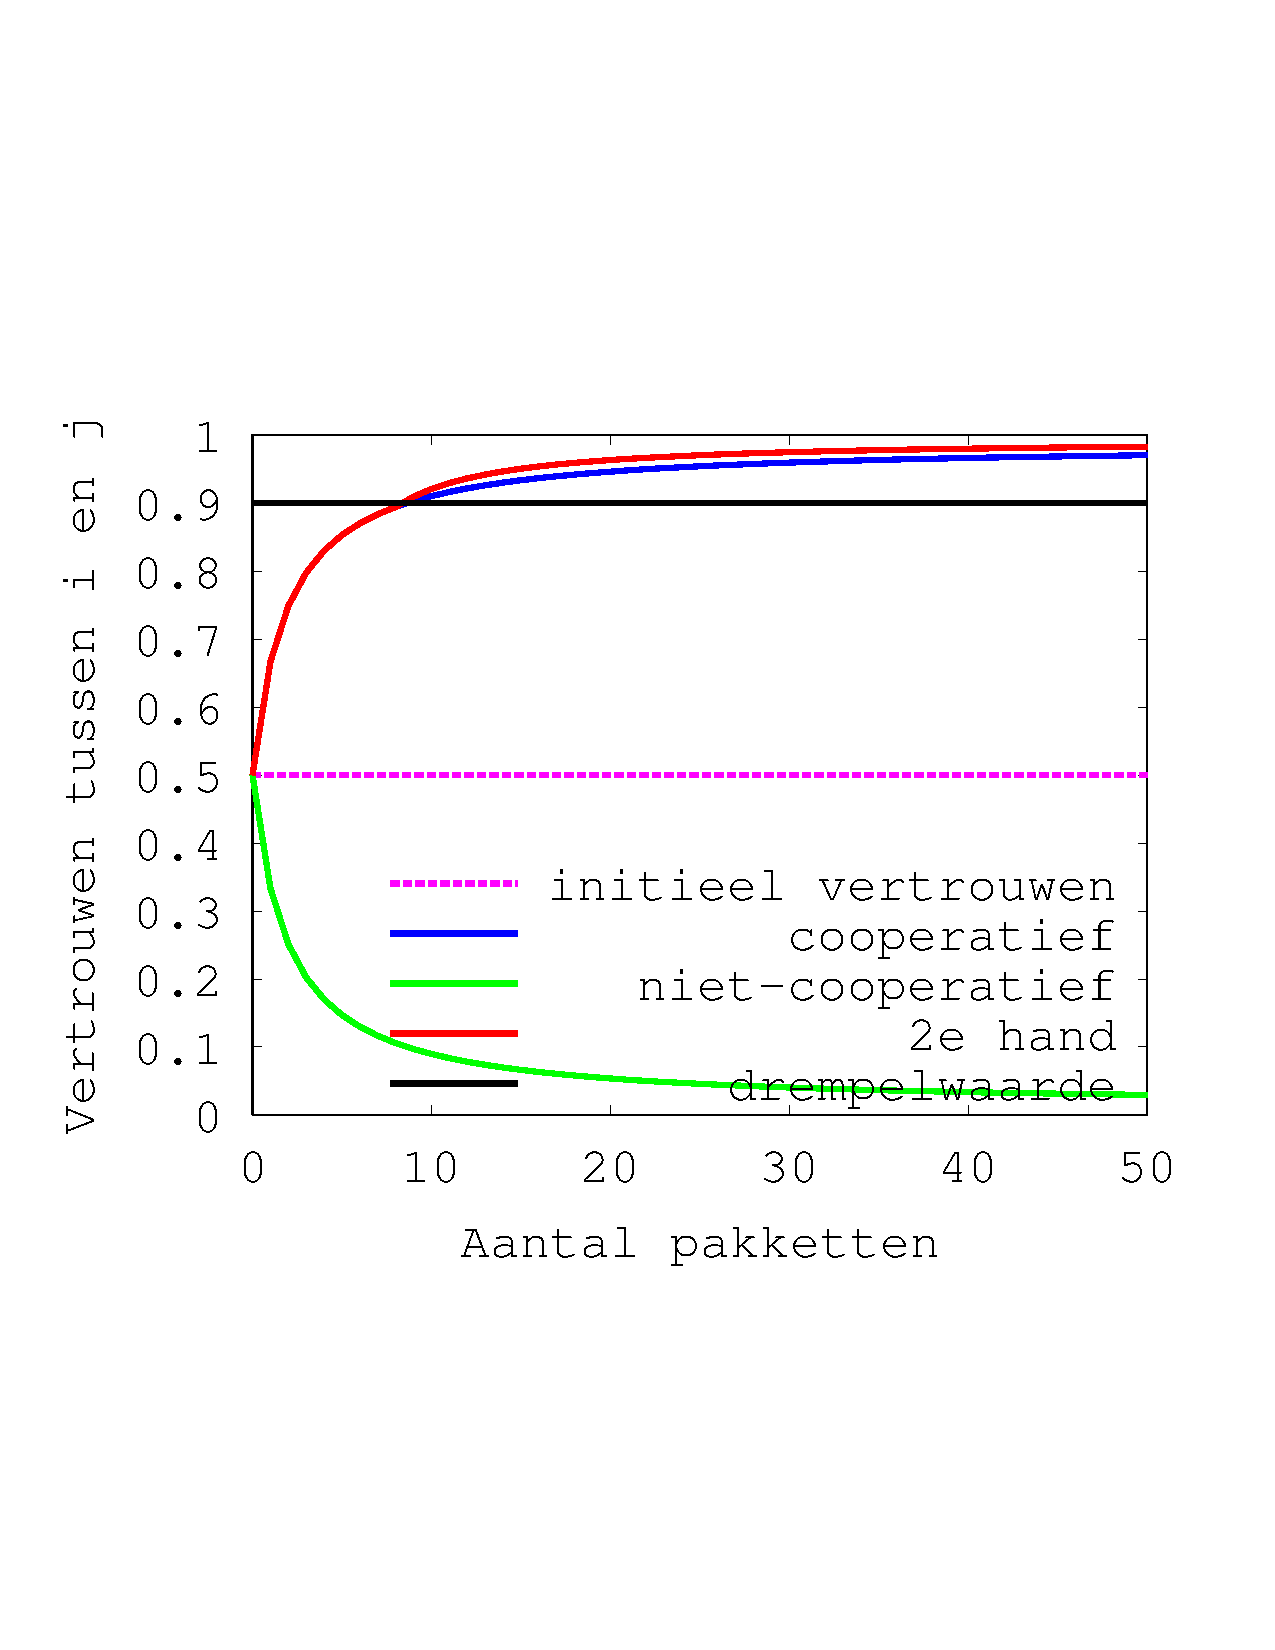
\includegraphics[width=.9\linewidth]{./resources/reputation-paper.pdf}
  \caption{Co\"operatieve en niet-co\"operatieve knopen}
  \label{fig:reputation-paper}
\end{subfigure}
\begin{subfigure}{.49\textwidth}
  \centering
  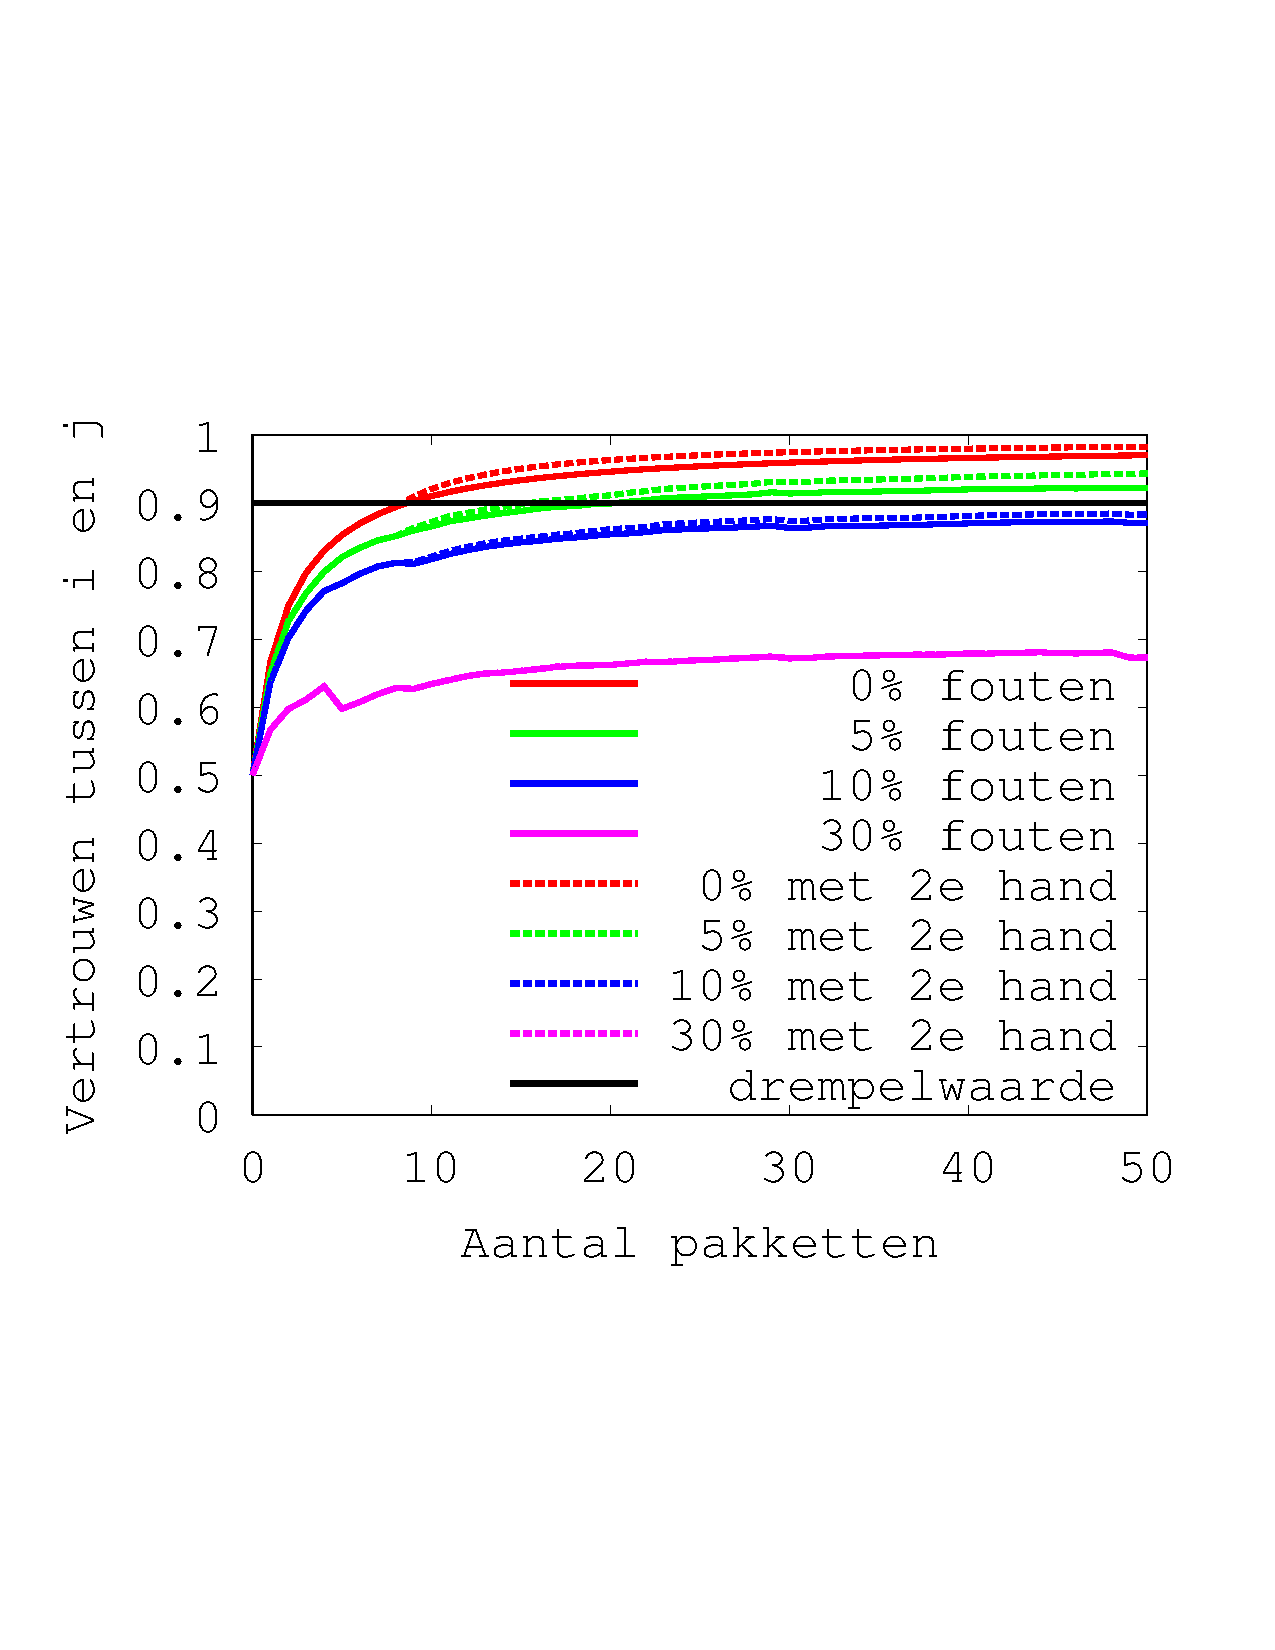
\includegraphics[width=.9\linewidth]{./resources/reputation-with-failure.pdf}
  \caption{Falende knopen (100 simulaties)}
  \label{fig:reputation-with-failure}
\end{subfigure}
\caption{Impact van falende knopen op evolutie van vertrouwen}
\label{fig:reputation-paper-with-failure}
\end{figure}

Deze eigenschap kan echter misbruikt worden zoals aangetoond wordt in figuur
\ref{fig:reputation-with-failure}. Stel dat een knoop $j$ te kampen heeft met
falende hardware, waardoor 5\% van zijn transmissies verloren gaan en daarom
ook niet opgemerkt kunnen worden door andere knopen.

We merken op dat deze knoop, zelfs met 5\% niet-co\"operatieve observaties, na
een twintigtal observaties toch boven de drempelwaarde uitkomt en door de
beschouwende knoop aanvaard wordt als betrouwbaar.

Vanuit een operationeel standpunt gezien is dit in eerste instantie een
positief effect. Indien een knoop \emph{slechts} 5\% faalt zal deze toch als
co\"operatief beschouwd worden en de goede werking van het netwerk niet
fundamenteel in het gedrang brengen - vanuit een inbraakdetectie-oogpunt gezien.

Maar stel dat deze 5\% niet-co\"operatieve acties geen falen zijn en dat de
doorgestuurde boodschappen niet verloren gaan, maar met opzet lichtjes
gewijzigd worden. 5\% kan een significante vertekening van metingen van een
netwerk betekenen en zo de werking van het hele netwerk ondermijnen.

Figuur \ref{fig:reputation-malicious} gaat slechts een kleine stap verder en
toont het effect van falende (of malafide) knopen die pas falingen vertonen
nadat ze het vertrouwen hebben gekregen van een knoop. We merken op dat nu zelfs
10\% falingen zeer lang het vertrouwen kunnen behouden.

\begin{figure}[ht]
 \centering
 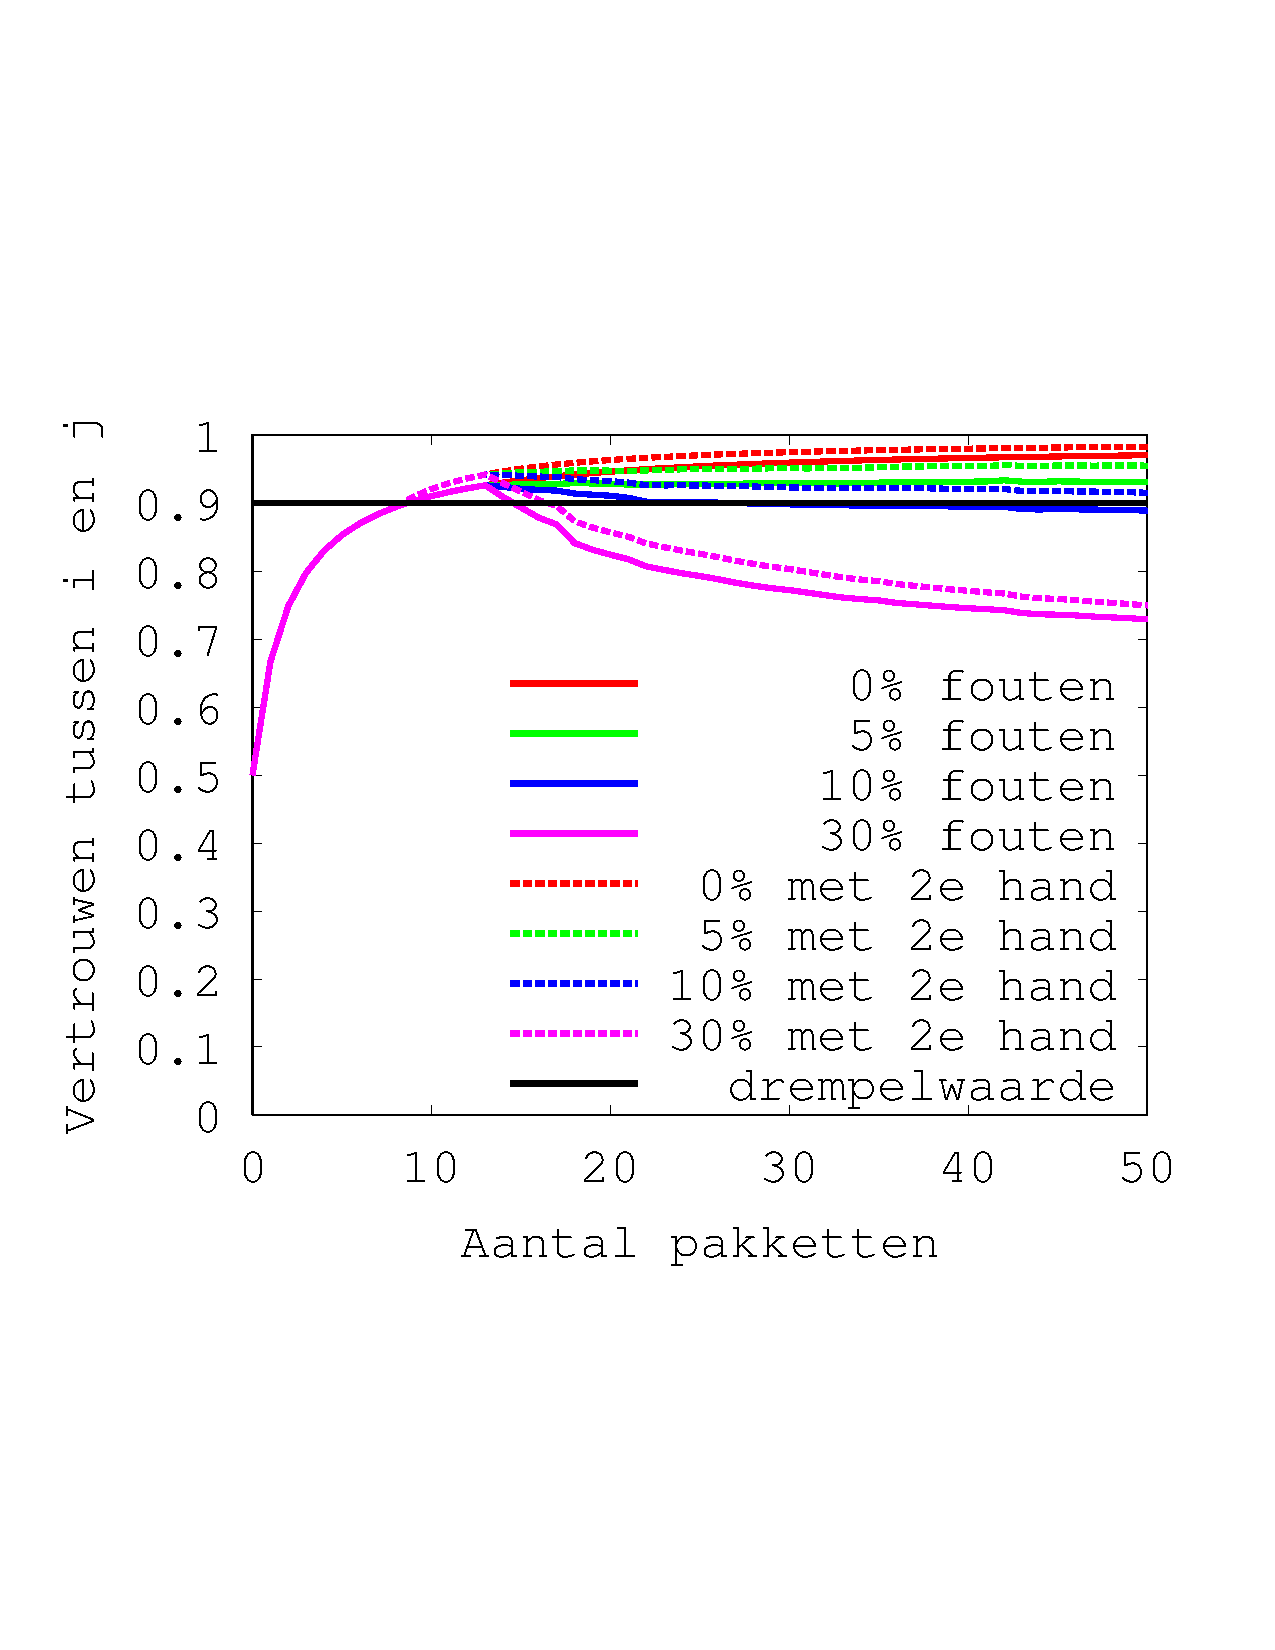
\includegraphics[width=.5\linewidth]{./resources/reputation-malicious.pdf}
 \caption{Falende knopen met vertraging van 15 pakketten (100 simulaties)}
 \label{fig:reputation-malicious}
\end{figure}

Dit elementaire voorbeeld toont duidelijk aan dat het vaststellen van een
reputatie op basis van externe observaties een zeer delicaat onderwerp is dat
zeer gevoelig is voor manipulatie op basis van kennis van de interne
parameters. Dit laatste is dan weer net \'e\'en van d\'e problemen waar
draadloze sensornetwerken mee kampen omdat knopen vrij eenvoudig kunnen
weggenomen, ge\"inspecteerd, gewijzigd en teruggeplaatst worden.

%!TEX root=masterproef.tex
\subsection{Co\"operatieve algoritmen}
\label{subsection:cooperation}

Het detecteren van abnormaal gedrag, dat op zijn beurt een indicatie kan zijn
van een (poging tot) inbraak, door \'e\'en knoop is \'e\'en ding. Als netwerk
van knopen tot een consensus komen en met meer zekerheid een verdachte knoop
uitsluiten is een heel ander ding.

Een veel voorkomend onderwerp daarom is dat van co\"operatie tussen knopen om
in overleg te bepalen of en welke andere knoop uitgesloten moet worden uit het
netwerk. In \cite{krontiris2009cooperative} wordt hiertoe eerst langs een
theoretische weg gezocht naar de nodige en voldoende voorwaarden voor
inbraakdetectie. Vervolgens wordt er een praktisch omkaderend algoritme
voorgesteld om op co\"operatieve manier aan inbraak detectie te doen.

Zowel het theoretische model als het praktische algoritme vormen een
interessante bron van informatie. Het theoretische model kan helpen bij het
analyseren van andere co\"operatieve oplossingen en het praktische algoritme
biedt een algemeen raamwerk voor het implementeren van co\"operatieve
strategie\"en.

\subsubsection*{IDP}

Het theoretische model beschrijft het ``Intrusion Detection Problem'', IDP, aan
de hand van $S = \{ s_1, s_2, \dots s_n \}$, de set van sensoren in het netwerk,
$N(s)$, de set van buren van $s$ en $D(s)$, de set van knopen die door $s$
verdacht worden. Indien $|D(s)| = 1$, is de aanvaller ge\"identificeerd.

Enkele predicaten worden gedefinieerd als volgt: $source(q)$ geldt indien $q$
de aanvaller is, $honest(s) \iff \neg source(s)$, $expose_s(q) \iff D(s) = \{ q
\}$ ofwel $s$ verklaart dat $q$ de aanvaller is en $A(s) \iff D(s) \not= \{\}$
wat zoveel betekent als dat $s$ gealarmeerd is. De set van gealarmeerde buren
van een knoop $s$ wordt gedefinieerd als $AN(s) = \{ t | A(t) \wedge t \in N(s)
\}$ en de set van gealarmeerde buren die nuttig is voor een knoop $s$ wordt dan
uitgedrukt als $\tilde{AN}(q,s) = AN(q) \backslash \{s\}$.

Het IDP wordt vervolgens gedefinieerd als het vinden van een algoritme dat
voldoet aan de eigenschappen van correctheid: $\forall s \in S : honest(s)
\wedge expose_s(s') \implies A(s) \wedge source(s')$ en eindigheid: bij een
aanval zullen na een tijd alle eerlijke knopen in de gealarmeerde set een knoop
verdenken.

Twee condities worden voorgesteld: de ``Intrusion Detection Condition'' of IDC
en de ``Neighbourhood Conditions'' of NC. Indien aan minstens \'e\'en van deze
condities voldaan is, is het IDP oplosbaar.

De IDC wordt beschreven als $\forall p,q \in S : source(q) \implies
\tilde{AN}(p,q) \not= \tilde{AN}(q,p)$. Dit drukt uit dat geen enkele andere
knoop een zelfde gealarmeerde buurt kan hebben als de aanvaller.

De NC worden beschreven door ``\emph{alle buren van een aanvaller zijn
gealarmeerd}'' ($NC_1$) en ``\emph{indien twee of meer knopen verdacht zijn door
een meerderheid van knopen, hebben de eerlijke knopen niet-gealarmeerde buren}''
($NC_2$).

Figuur \ref{fig:idp-examples} illustreert het IDP en toepassing van IDC en NC
aan de hand van enkele voorbeelden:

\begin{figure}[ht]
\centering
\begin{subfigure}{.49\textwidth}
  \centering
\[ \entrymodifiers={}
 \xymatrix@!=0.75pc {
 *{}                                      & *{} & *-=++[o][F]{b} \ar@<0.7ex>[dll]\\
 *-=++[F]{a} \ar@<0.7ex>[urr] \ar@<0.7ex>[drr]& *{} & *{}                        \\
 *{}                                      & *{} & *-=++[o][F]{c} \ar@<0.7ex>[ull]\\
 }
\]
  \caption{}
  \label{fig:idp-examples-1}
\end{subfigure}
\begin{subfigure}{.49\textwidth}
  \centering
\[ \entrymodifiers={}
 \xymatrix@!=0.75pc {
 *{} & *{} & *{}                                      & *{} & *-=++[o][F]{b} \ar@<0.7ex>[dll] \ar[dd]\\
 *-=++[o][F]{d} \ar@<0.7ex>[rr] & *{} & *-=++[F]{a} \ar@<0.7ex>[ll] \ar@<0.7ex>[urr] \ar@<0.7ex>[drr]& *{} & *{} \\
 *{} & *{} & *{}                                      & *{} & *-=++[o][F]{c} \\
 }
\]
  \caption{}
  \label{fig:idp-examples-2}
\end{subfigure}
\caption{Voorbeelden van de toepassing van IDC en NC. Vierkante knopen zijn
aanvallers, omcirkelde knopen zijn gealarmeerd. $x \rightarrow y$ betekent dat
knoop $x$ knoop y verdenkt.}
\label{fig:idp-examples}
\end{figure}

De situatie in figuur \ref{fig:idp-examples-1} voldoet niet aan de IDC omdat
$\tilde{AN}(a,b) = \{c\} = \tilde{AN}(b,a)$. Maar in dit geval is wel voldaan
aan beide NC. Het IDP kan in dit geval opgelost worden aan de hand van een
deterministisch algoritme. Omdat er slechts \'e\'en knoop het hoogste aantal
verdenkingen op zijn naam heeft staan, kunnen knopen $b$ en $c$ eenvoudig
beslissen dat knoop $a$ de aanvaller is.

Figuur \ref{fig:idp-examples-2} toont een situatie waar de IDC wel voldaan is
want $\tilde{AN}(q,r) = \{s\} \not= \tilde{AN}(r,q) = \{\}$. Er zijn echter nu
twee knopen met een meerderheid aan verdenkingen: $a$ en $c$. Vanuit het
standpunt van knoop $b$ moet dus knoop $a$ of knoop $d$ valse aantijgingen
verspreiden. Als \'e\'en van deze knopen de aanvaller is, dan moet
$\tilde{AN}(a,d) \not= \tilde{AN}(d,a)$, anders is niet voldaan aan de IDC. Dit
impliceert tevens dat $\exists x : A(x) \wedge ( x \not\in N(a) \vee x \not\in
N(d) )$, ofwel dat er een knoop bestaat die gealarmeerd is, maar geen buur is
van de andere eerlijke knoop van de twee verdachte knopen. In dit geval zijn
knopen $b$ en $d$ inderdaad geen buren, maar beide verdenken knoop $a$.

\subsubsection*{Algoritme}
\label{subsubsection:cooperation-algorithm}

Naast een theoretisch model, introduceren \cite{krontiris2009cooperative}
tevens een algoritme dat kan dienen als raamwerk voor co\"operatieve
inbraakdetectie. Het algoritme bestaat uit vier tot vijf fasen: initialisatie,
stemming, publicatie van gebruikte sleutels, ontmaskeren van de aanvaller en
optioneel het inroepen van informatie uit de externe kring. Het is in essentie
een implementatie van het Guy Fawkes protocol, beschreven in
\cite{anderson1998new}, dat toelaat om een reeks van berichten te authenticeren
op basis van \'e\'en initi\"eel gedeelde sleutel.

Tijdens de initialisatie fase krijgt elke knoop een unieke sleutel, $K_l$. Aan
de hand van deze sleutel wordt een \'e\'en-richtingsketting van langte $l$
gemaakt van sleutels door het toepassen van bv. SHA1 \cite{rfc:3174} hashing
toe te passen: $\{K_0, K_1, \dots K_{l-1}\}$ waarbij $\forall k \in [1..l] :
K_{k-1} = SHA1(K_k)$. Daarnaast worden ook naburige knopen gezocht tot twee
knopen ver en wordt sleutel $K_0$ gecommuniceerd aan al deze buren. De
volledige initialisatie fase wordt verondersteld te gebeuren zonder
mogelijkheid tot inbraken.

Tijdens de stemming brengen alle knopen een stem uit van de vorm $m_v(s),$ $
MAC_{K_j}(m_v(s))$. $m_v(s)$ bestaat uit een lijst van knopen die door knoop
$s$ beschouwd worden als mogelijke aanvallers, of uitgedrukt aan de hand van
het theoretische model: $m_v(s) = D(s)$. De $MAC_{K_j}()$ functie is een zgn.
\emph{Message Authentication Code} \cite{rfc:2104} en wordt meestal berekend
door het toepassen van een \'e\'en-richtings-hashfunctie toe te passen op de
boodschap. Typisch wordt er aan de boodschap een unieke, wederzijds gekende
identificatie toegevoegd, zodat de ontvanger van een boodschap deze
handtekening ook kan berekenen en vergelijken met het origineel. In dit geval
wordt $K_j$ gebruikt, waarbij $j$ de volgende indexwaarde krijg uit lijst van
beschikbare sleutels.

Een dergelijke boodschap kan op ogenblik van verzending door geen enkele andere
knoop gevalideerd worden. De enige sleutel die zij tot op dat ogenblik kennen
is de vorige en de vorige is net het resultaat van een SHA1 operatie op de
volgende. Dit betekent dat ook een mogelijke aanvaller niet in staat is om de
boodschap te wijzigen.

Pas wanneer de knopen elkaars stemmen hebben ontvangen, wordt de gebruikte
sleutel vrijgegeven in de publicatie fase. Op dit ogenblik kunnen de knopen de
eerder verstuurde stemmen valideren. Ze kunnen eerst controleren of de
gepubliceerde sleutel inderdaad de juiste is. Immers, door het toepassen van
SHA1 op deze sleutel, moeten zij de huidige gekende sleutel bekomen. Na
validatie van de nieuwe sleutel, kan ook de boodschap gevalideerd worden.

Nu alle knopen de stemmen van alle knopen ontvangen hebben en zeker zijn dat de
stemmen authentiek zijn, kan met \'e\'enzelfde algoritme door alle knopen de
aanvaller bepaald worden tijdens de ontmaskering fase.

Het is echter mogelijk dat er meerdere knopen zijn met eenzelfde aantal stemmen
zijn, iets dat typisch overeenkomt met een gelijke samenstelling van
gealarmeerde buren, wanneer de IDC niet kan gerealiseerd worden. Onder
voorbehoud dat aan de NC wel voldaan wordt, kan door het inroepen van de niet
gealarmeerde buren van de gealarmeerde knopen. Deze zullen op hun beurt nagaan
of de knopen die verdacht worden, buren zijn en dan aangeven dat zij hen
\emph{niet} verdenken. Aan de hand van deze informatie kunnen de eerder
gealarmeerde knopen hun beslissing verder staven.

Het algoritme is een betrekkelijk eenvoudig raamwerk voor een co\"operatieve
aanpak, waarbij knopen lokaal beslissen welke andere knopen ze verdenken en
vervolgens gedistribueerd, gezamenlijk trachten tot een consensus te komen
welke van de de verdachte knopen effectief de aanvaller is.

De kracht van dit raamwerk en het succes ervan hangt natuurlijk sterk af van de
lokale detectie mogelijkheden van de knopen en de accuraatheid hiervan.

\subsubsection*{Risico's}

Het voorbeeld in figuur \ref{fig:idp-examples-2} beslaat een zeer beperkte
scope. We moeten voorzichtig zijn om hier niet te snel tot conclusies te komen
die in een ruimere situatie misschien een totaal verkeerd beeld zouden kunnen
opleveren. Figuur \ref{fig:sinkhole-ripple} toont essentieel het zelfde
voorbeeld als dat van \ref{fig:idp-examples-2}, maar nu met meer knopen rondom
het initi\"ele voorbeeld.

Het routering algoritme is gebaseerd op de totale kost van het pad naar het
basisstation en komt daarmee overeen met het MultiHopLQI routering algoritme
beschreven in o.a. \cite{krontiris2008launching}. In dit werk wordt ook de zgn.
\emph{Sinkhole Attack} voorgesteld. We nemen deze aanval als voorbeeld.

\begin{figure}[ht]
\centering
\begin{subfigure}{.49\textwidth}
  \centering
\[ \entrymodifiers={-=++[o][F]}
 \xymatrix@!=0.75pc {
*{} & e \ar@{->}[l]_{100} & *{} & f \ar@{->}[ll]_{50}   & *{} \\
*{} & *{} & *{} &  *{} & b \ar@{->}[lu]_{35} \ar@{.}[ld]_{20} \ar@{.}[dd]^{30}  \\
*{} & d \ar@{->}[uu]^{75} \ar@{.}[dd]_{75}  & *{} &    a \ar@{->}[lluu]_{80} \ar@{.}[lldd]^{80} \ar@{.}[ll]_{50} & *{} \\
*{} & *{} & *{} &  *{} & c \ar@{.}[lu]^{20} \ar@{->}[ld]^{35} \\
*{} & h \ar@{->}[l]^{105}  & *{} &  g \ar@{->}[ll]^{50}  & *{} \\
  }
\]
  \caption{Initi\"ele topologie, routes en kosten}
  \label{fig:sinkhole-ripple-1}
\end{subfigure}
\begin{subfigure}{.49\textwidth}
  \centering
\[ \entrymodifiers={-=++[o][F]}
 \xymatrix@!=0.75pc {
*{} & e \ar@{->}[l]_{100} & *{} & f \ar@{->}[ll]_{50}   & *{} \\
*{} & *{} & *{} &  *{} & b \ar@{.}[lu]_{35} \ar@{~>}[ld]_{20} \ar@{.}[dd]^{30}  \\
*{} & *-=++[F]{d} \ar@{~>}[l]^{50} \ar@{.}[uu]^{75} \ar@{.}[dd]_{75}  & *{} &    a \ar@{.}[lluu]_{80} \ar@{.}[lldd]^{80} \ar@{~>}[ll]_{50} & *{} \\
*{} & *{} & *{} &  *{} & c \ar@{~>}[lu]^{20} \ar@{.}[ld]^{35} \\
*{} & h \ar@{->}[l]^{105}  & *{} &  g \ar@{->}[ll]^{50}  & *{} \\
  }
\]
  \caption{Knoop $d$ kondigt ``betere'' route aan.}
  \label{fig:sinkhole-ripple-2}
\end{subfigure}
\caption{Voorbeeld van het theoretische risico dat kan leiden tot een verkeerde
identificatie van de echte aanvaller.}
\label{fig:sinkhole-ripple}
\end{figure}

Stel dat knoop $d$ een \emph{Sinkhole Attack} uitvoert door een zeer lage kost
te adverteren. Hierdoor zal knoop $a$ geneigd zijn om zijn route aan te passen.
Hierdoor zal deze op zijn beurt een veel voordeligere route adverteren en
zullen ook knopen $b$ en $c$ hun route wijzigen en nu hun gegevens via knoop
$a$ versturen.

Ten gevolge van deze route updates is het mogelijk dat een lokale detector voor
de \emph{Sinkhole Attack} op knopen $a$ en $b$ zal in werking treden. Hierbij
kunnen de knopen slechts hun volledige buurt beschuldigen, omdat het niet
mogelijk is om te detecteren wie de valse boodschappen effectief verstuurd
heeft. Indien de aanvallende knoop $d$ nu ook selectief zijn naburige knoop $a$
beschuldigd, bekomen we dezelfde situatie als in figuur
\ref{fig:idp-examples-2}, echter nu met mogelijk een verkeerd
ge\"identificeerde aanvaller.

Dit voorbeeld is, net zoals de vele andere beschreven voorbeelden, uitermate
specifiek en dient louter ter illustratie van het fragiele karakter van een
co\"operatief algoritme. Desalniettemin bieden de concepten en het omkaderende
algoritme ge\"introduceerd in \cite{krontiris2009cooperative} een goed
uitgangspunt om te hanteren bij het beschrijven en implementeren van inbraak
detectie mechanismen.

\subsubsection*{Groeperen}
\label{subsubsection:grouping}

Een andere aanpak van co\"operatieve algoritmen vertrekt van het groeperen van
knopen. Deze aanpak wordt toegepast door \cite{li2008group}. Groepering gebeurt
op basis van nabijheid en tracht sensoren te groeperen die door hun locatie
gelijkaardige meetwaarden zouden moeten opmeten. De auteurs stellen hiervoor
een dynamisch $\delta$-algoritme voor.

Metingen van knopen kunnen nu binnen de groep met elkaar vergeleken worden, en
op statistische wijze kunnen afwijkende resultaten (zie ook sectie
\ref{subsection:anomaly}) nu eventueel beschouwd worden als abnormaal gedrag en zo
gerapporteerd worden.

%!TEX root=masterproef.tex
\subsection{Attesteren van software}
\label{subsection:attestation}

Het voorbeeld uit sectie \ref{section:node-capture} toonde al aan dat zelfs het
vluchtige geheugen van een knoop niet veilig is. Als een aanvaller in staat is
om ongemerkt de programma-code van een knoop te bekomen, alsook alle gegevens
die alleen tijdens uitvoering in het geheugen, dan kan deze aanvaller deze code
aanpassen zodat de werking ogenschijnlijk ongewijzigd is, maar dat hij toch
controle heeft over de werking en zo het hele netwerk kan be\"invloeden.

Een zeer logische onderzoeksvraag dient zich al snel aan: ``\emph{Is het
mogelijk om wijzigingen aan het programma van een knoop in het netwerk vast te
stellen?}''. Deze vraag wordt onderzocht binnen het domein van software
attestatie.

\subsubsection*{Werking}

Alle bestaande vormen van software attestatie maken gebruik van een protocol
gebaseerd op het challenge response principe. Als men de integriteit van een
knoop wil vast stellen, zal men aan deze knoop een verzoek sturen om een unieke
samenvatting te maken van zijn inhoud door middel van een cryptografische
hashfunctie, een \emph{checksum}.

De vaststeller beschikt zelf over een versie van de inhoud van de knoop en kan
dezelfde unieke samenvatting berekenen. Door in het initi\"ele verzoek een
\'e\'enmalig te gebruiken code mee te geven, een zgn. \emph{nonce}, en deze
deel te laten uitmaken van de inhoud, kunnen verschillende verzoeken telkens
met een ander, unieke samenvatting beantwoord worden en wordt kan deze
samenvatting niet op voorhand gekend en berekend worden. Figuur
\ref{fig:attestation-process} geeft een overzicht van de werking van software
attestatie en illustreert hoe een wijziging door een aanvaller zich propageert.

\begin{figure}
  \centering
  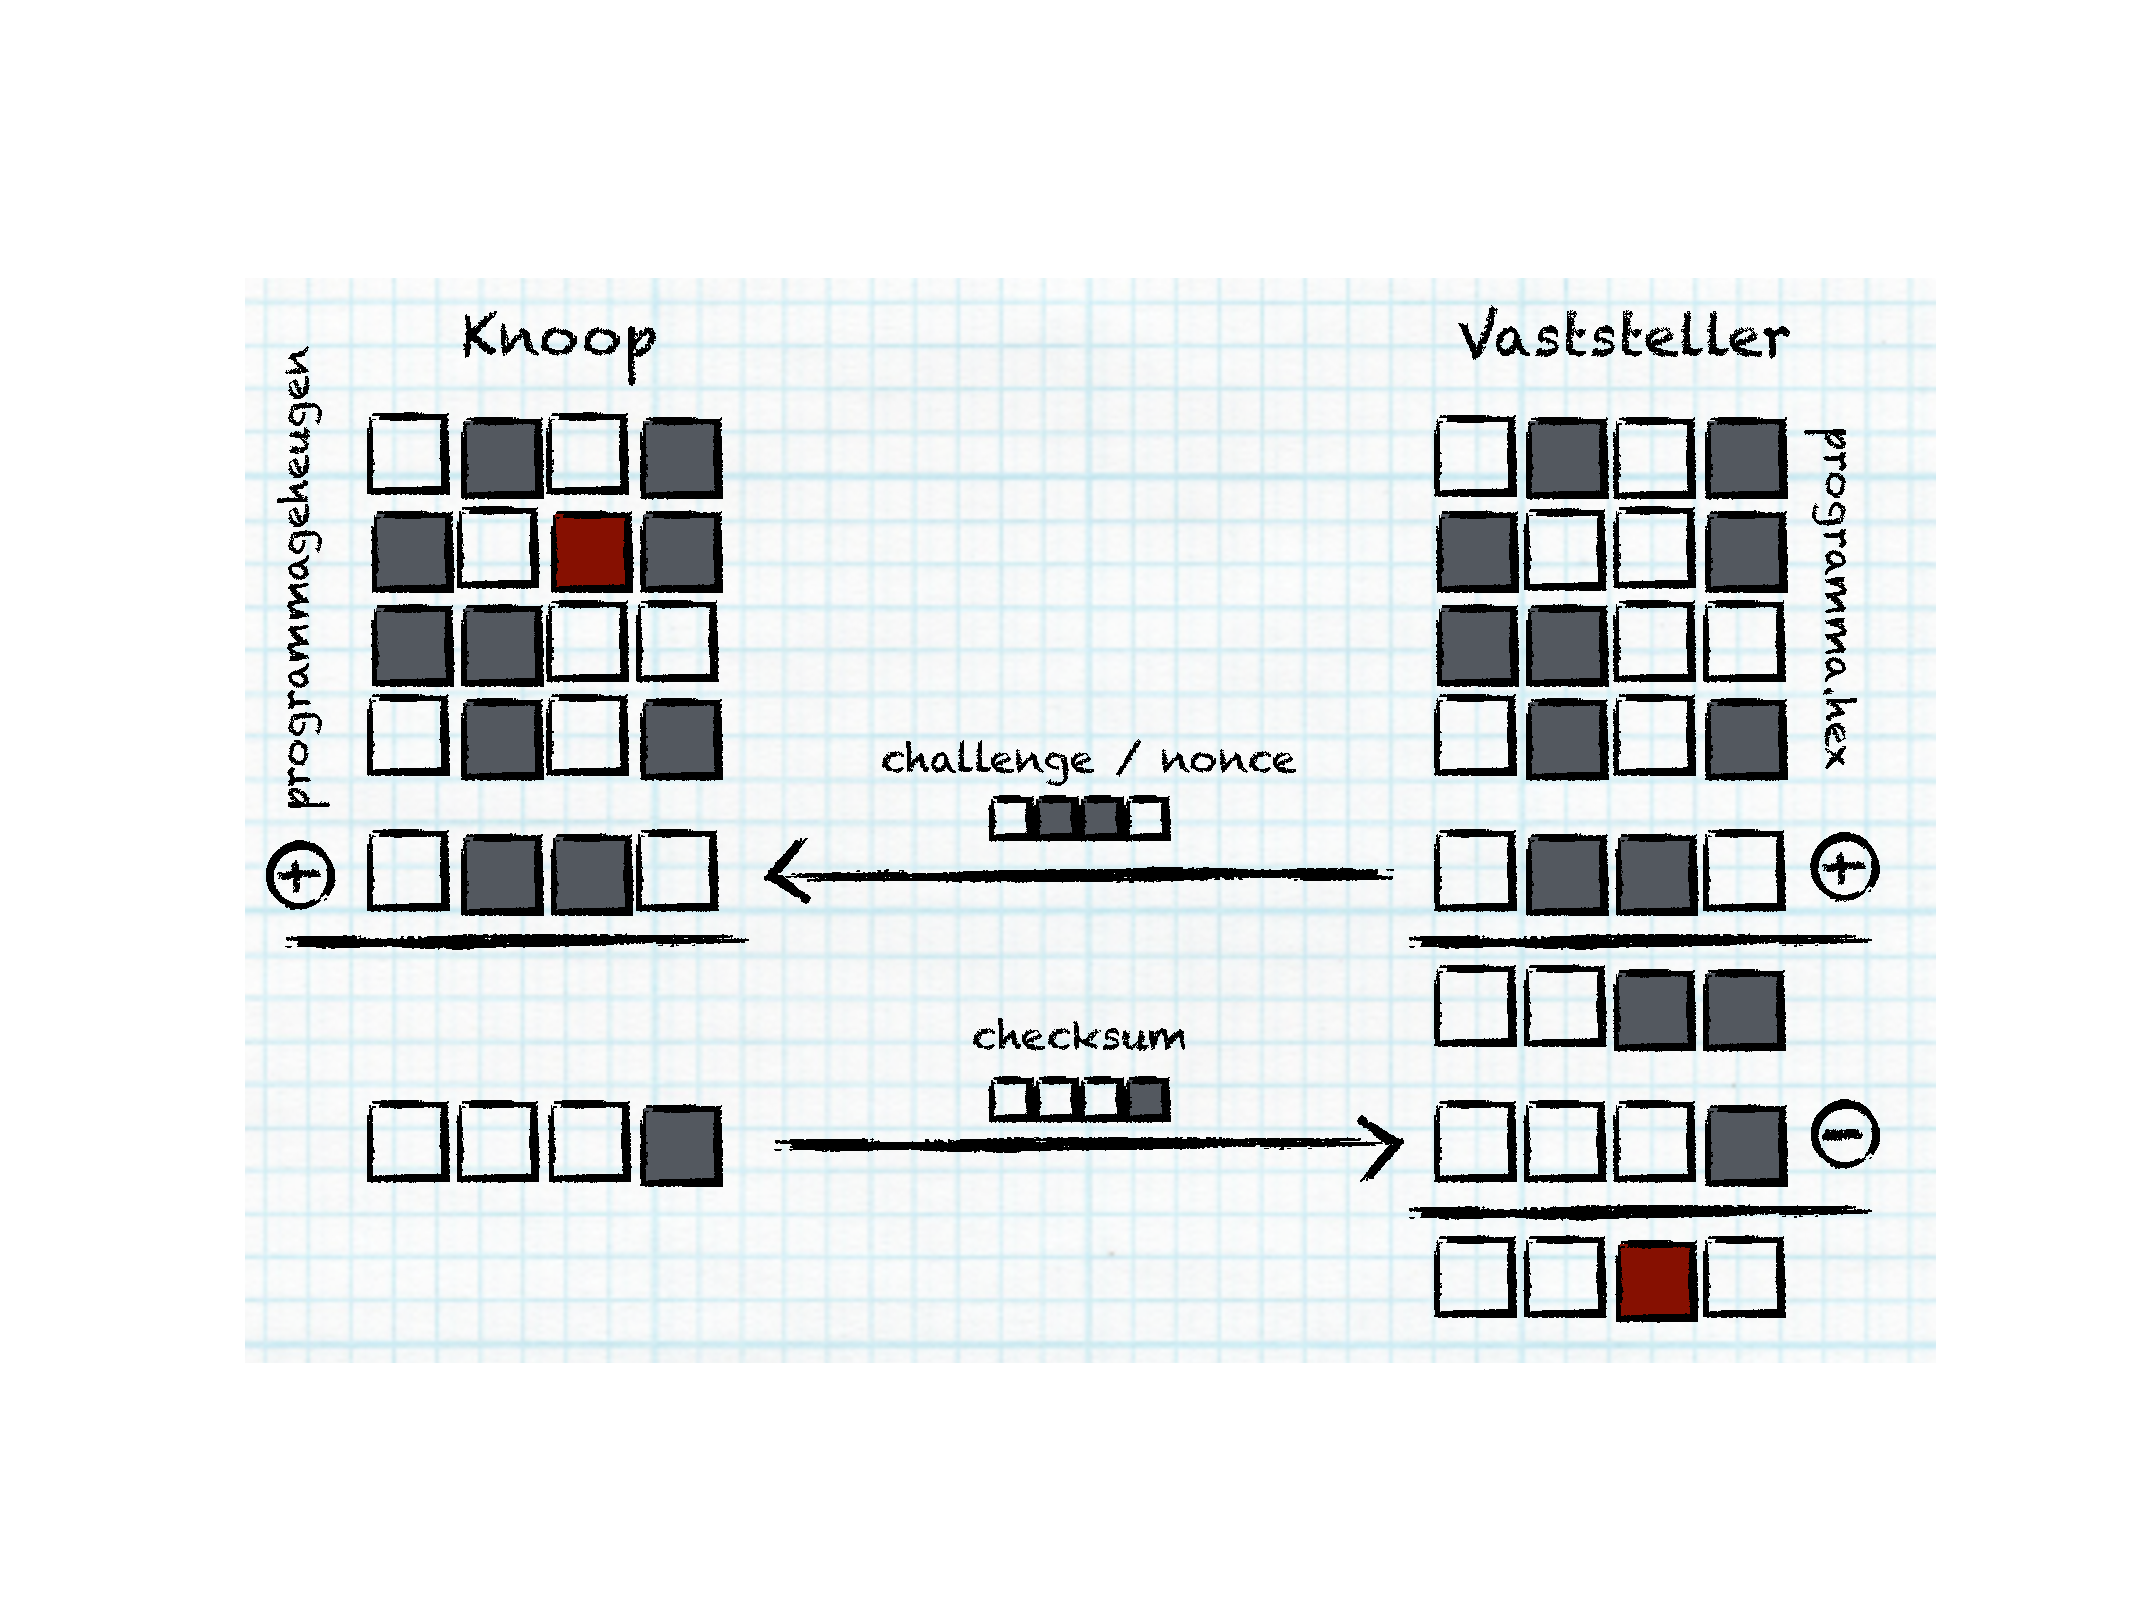
\includegraphics[width=0.9\linewidth]{resources/attestation-process.pdf}
  \caption{De werking van software attestatie: een aanvaller heeft een
  wijziging kunnen aanbrengen in de programma code op een knoop. Deze wijziging
  propageert zich in de \emph{checksum} en wordt door de vaststeller opgemerkt.}
  \label{fig:attestation-process}
\end{figure}

De inhoud waarvan een samenvatting gemaakt wordt is typisch de programma code
die op de knoop ge\"installeerd werd. Indien een aanvaller deze code kon
wijzigen, zou de samenvatting niet langer overeenkomen met die opgesteld door
de vaststeller en kan deze laatste besluiten om deze gewijzigde code niet te
vertrouwen en de knoop uit te sluiten.

\subsubsection*{Implementaties}

SWATT werd voorgesteld in \cite{seshadri2004swatt}. Het is een attestatie
procedure die een \emph{checksum} berekent over nagenoeg alle geheugenlocaties,
echter wel in willekeurige volgorde. Anderzijds houdt SWATT ook rekening houdt
met de tijd die de attestatie routine op de knoop nodig heeft om de
\emph{checksum} te berekenen. Indien een aanvaller code zou toevoegen om de
werking van de attestatie routine te verstoren, zou op te merken zijn in een
vertraging.

Met SCUBA in \cite{seshadri2006scuba} en SAKE in \cite{seshadri2008sake} werd
verder gebouwd op de SWATT techniek met het oog op een beveiligde distributie
van programma code en het veilig uitwisselen van sleutels. Samen met SCUBA en
SAKE werd ook \emph{Indisputable Code Execution} of ICE ge\"introduceerd. Daar
waar SWATT gericht is op inhoudelijke integriteit, voegt ICE hieraan ook de
garantie van een niet aangetaste uitvoering van programma's aan toe en laat het
toe om beperkte regio's van het geheugen te benaderen.

Op deze manier kan nu bovenop de attestatie van het geheugen van een knoop, nu
ook functionaliteit aangeroepen worden, waarvan de werking ook gegarandeerd
veilig is. Het installeren van nieuwe code en het uitwisselen van gedeelde
geheimen wordt op die manier mogelijk.

ICE realiseert dit door een \emph{checksum} te berekenen over de geheugenregio
waar de attestatie routine zich bevindt, alsook over de regio waar het uit te
voeren programma staat en van de staat van de processor. Hierdoor ontstaat er
een garantie dat de attestatie correct verloopt, dat het uit te voeren
programma geen onbekende code bevat en dat de omgeving waarin de attestatie en
het programma uitgevoerd worden gegarandeerd niet aangetast kan worden.

Een belangrijke eigenschap van de ICE techniek is dat de attestatie routine de
processor in een emph{veilige} staat brengt door geen interrupts toe te laten.
Hierdoor kan de werking van de attestatie routine niet onderbroken en gewijzigd
worden. Na correcte attestatie zal het geattesteerde programma in dezelfde
veilige omstandigheden als de ICE routine uitgevoerd worden.

\subsubsection*{Evaluatie}

De beweringen rond SWATT en ICE werden in \cite{castelluccia2009difficulty}
onder de loep genomen en verschillende manieren om deze vormen van
integriteits-controle te omzeilen werden voorgesteld. Ondanks het feit dat
verschillende interessante aspecten van de attestatie technieken werden
belicht, werden te snel veronderstellingen rond beide implementaties gemaakt en
werd in \cite{perrig2010refutation} een weerwoord gegeven.

Desalniettemin zijn de ontwijkingstechnieken die voorgesteld werden zeer
interessante voorbeelden van de mogelijkheden die een aanvaller heeft tegen
software attestatie. Het feit dat de op het eerste zicht inderdaad valabele
aanvallen toch nog fouten bevatten, biedt dan weer een ander interessant beeld
op de kwaliteiten van de voorgestelde technieken. We belichten ze in de
volgende paragrafen als inspiratiebron.

De fundamentele manier om de attestatie code te omzeilen bestaat er in om de
opgevraagde geheugenadressen te controleren en indien ze verwijzen naar
plaatsen waar zich niet-originele code bevindt, deze te herschrijven naar
adressen waar de originele code zich bevindt.

Aangezien het merendeel van het programma geheugen op een knoop typisch leeg
is, kan de aanvaller zijn benodigde code verbergen in zo'n stuk leeg geheugen.
Mits zorgvuldige keuze van deze locatie, kan het controleren van en verwijzen
naar een andere locatie zich beperken tot de manipulatie van \'e\'en enkele bit
in het adres. Deze techniek wordt ook wel een geheugen schaduwende aanval
genoemd.

Om het probleem van leeg programma geheugen en de bijhorende uitnodiging aan
het adres van de aanvaller om zich eenvoudig te kunnen verschuilen, aan te
pakken, stelelen o.a. \cite{yang2007distributed,seshadri2008sake} voor om dit
geheugen voor dat het op een knoop wordt geplaatst, op te vullen met
willekeurige waarden. Op deze manier heeft de aanvaller geen vrije ruimte om
zijn code in te plaatsen.

Ofschoon deze willekeurige data inderdaad zo kan opgesteld worden dat ze niet
kan verkleind worden, kan dit niet gegarandeerd worden van de eigenlijke
programma code. Deze kan typisch wel nog verkleind worden en in die vorm
opgeslagen worden, waardoor er mogelijk voldoende ruimte vrijkomt voor de code
van de aanvaller. Op het ogenblik van attestatie kan deze oorspronkelijke code
dan, indien nodig terug hersteld worden.

Indien deze eenvoudige technieken toch niet voldoende ruimte zouden bieden, kan
er nog altijd gekeken worden naar het data geheugen. We merken immers op dat
nagenoeg alle vormen van attestatie alleen toegepast worden op het programma
geheugen. Het data geheugen is immers te veranderlijk en kan niet volledig
gekend zijn door de vaststeller.

Hierdoor wordt dit data geheugen natuurlijk het volgende mogelijke
aandachtspunt voor de aanvaller. Ondanks het feit dat ook op een \mcu het data
geheugen veelal niet kan uitgevoerd worden, blijft het mogelijk om programma
code in het data geheugen op te slagen en te kopi\"eren naar het programma
geheugen.

De \emph{rootkit} voorgesteld in \cite{castelluccia2009difficulty} hanteert dit
principe. Door middel van de \emph{Return Operation Programming} (ROP)
techniek, o.a. beschreven in \cite{prandini2012return}, kan een aanvaller met
eerste haak bij aanvang van de attestatie code in het programma geheugen, zijn
eigen rootkit uit het programma geheugen laten verwijderen. Na deze operatie is
het programma geheugen opnieuw intact en zal de originele attestatie routine
een positief resultaat opleveren. Maar de eerste haak heeft er ook voor gezorgd
dat de bij terugkeer uit de attestatie routine een tweede haak geplaatst is die
op zijn beurt de rootkit en de initi\"ele haak opnieuw door middel van ROP
instructies installeert. Figuur \ref{fig:attestation-rootkit} toont deze
werking.

\begin{figure}
  \centering
  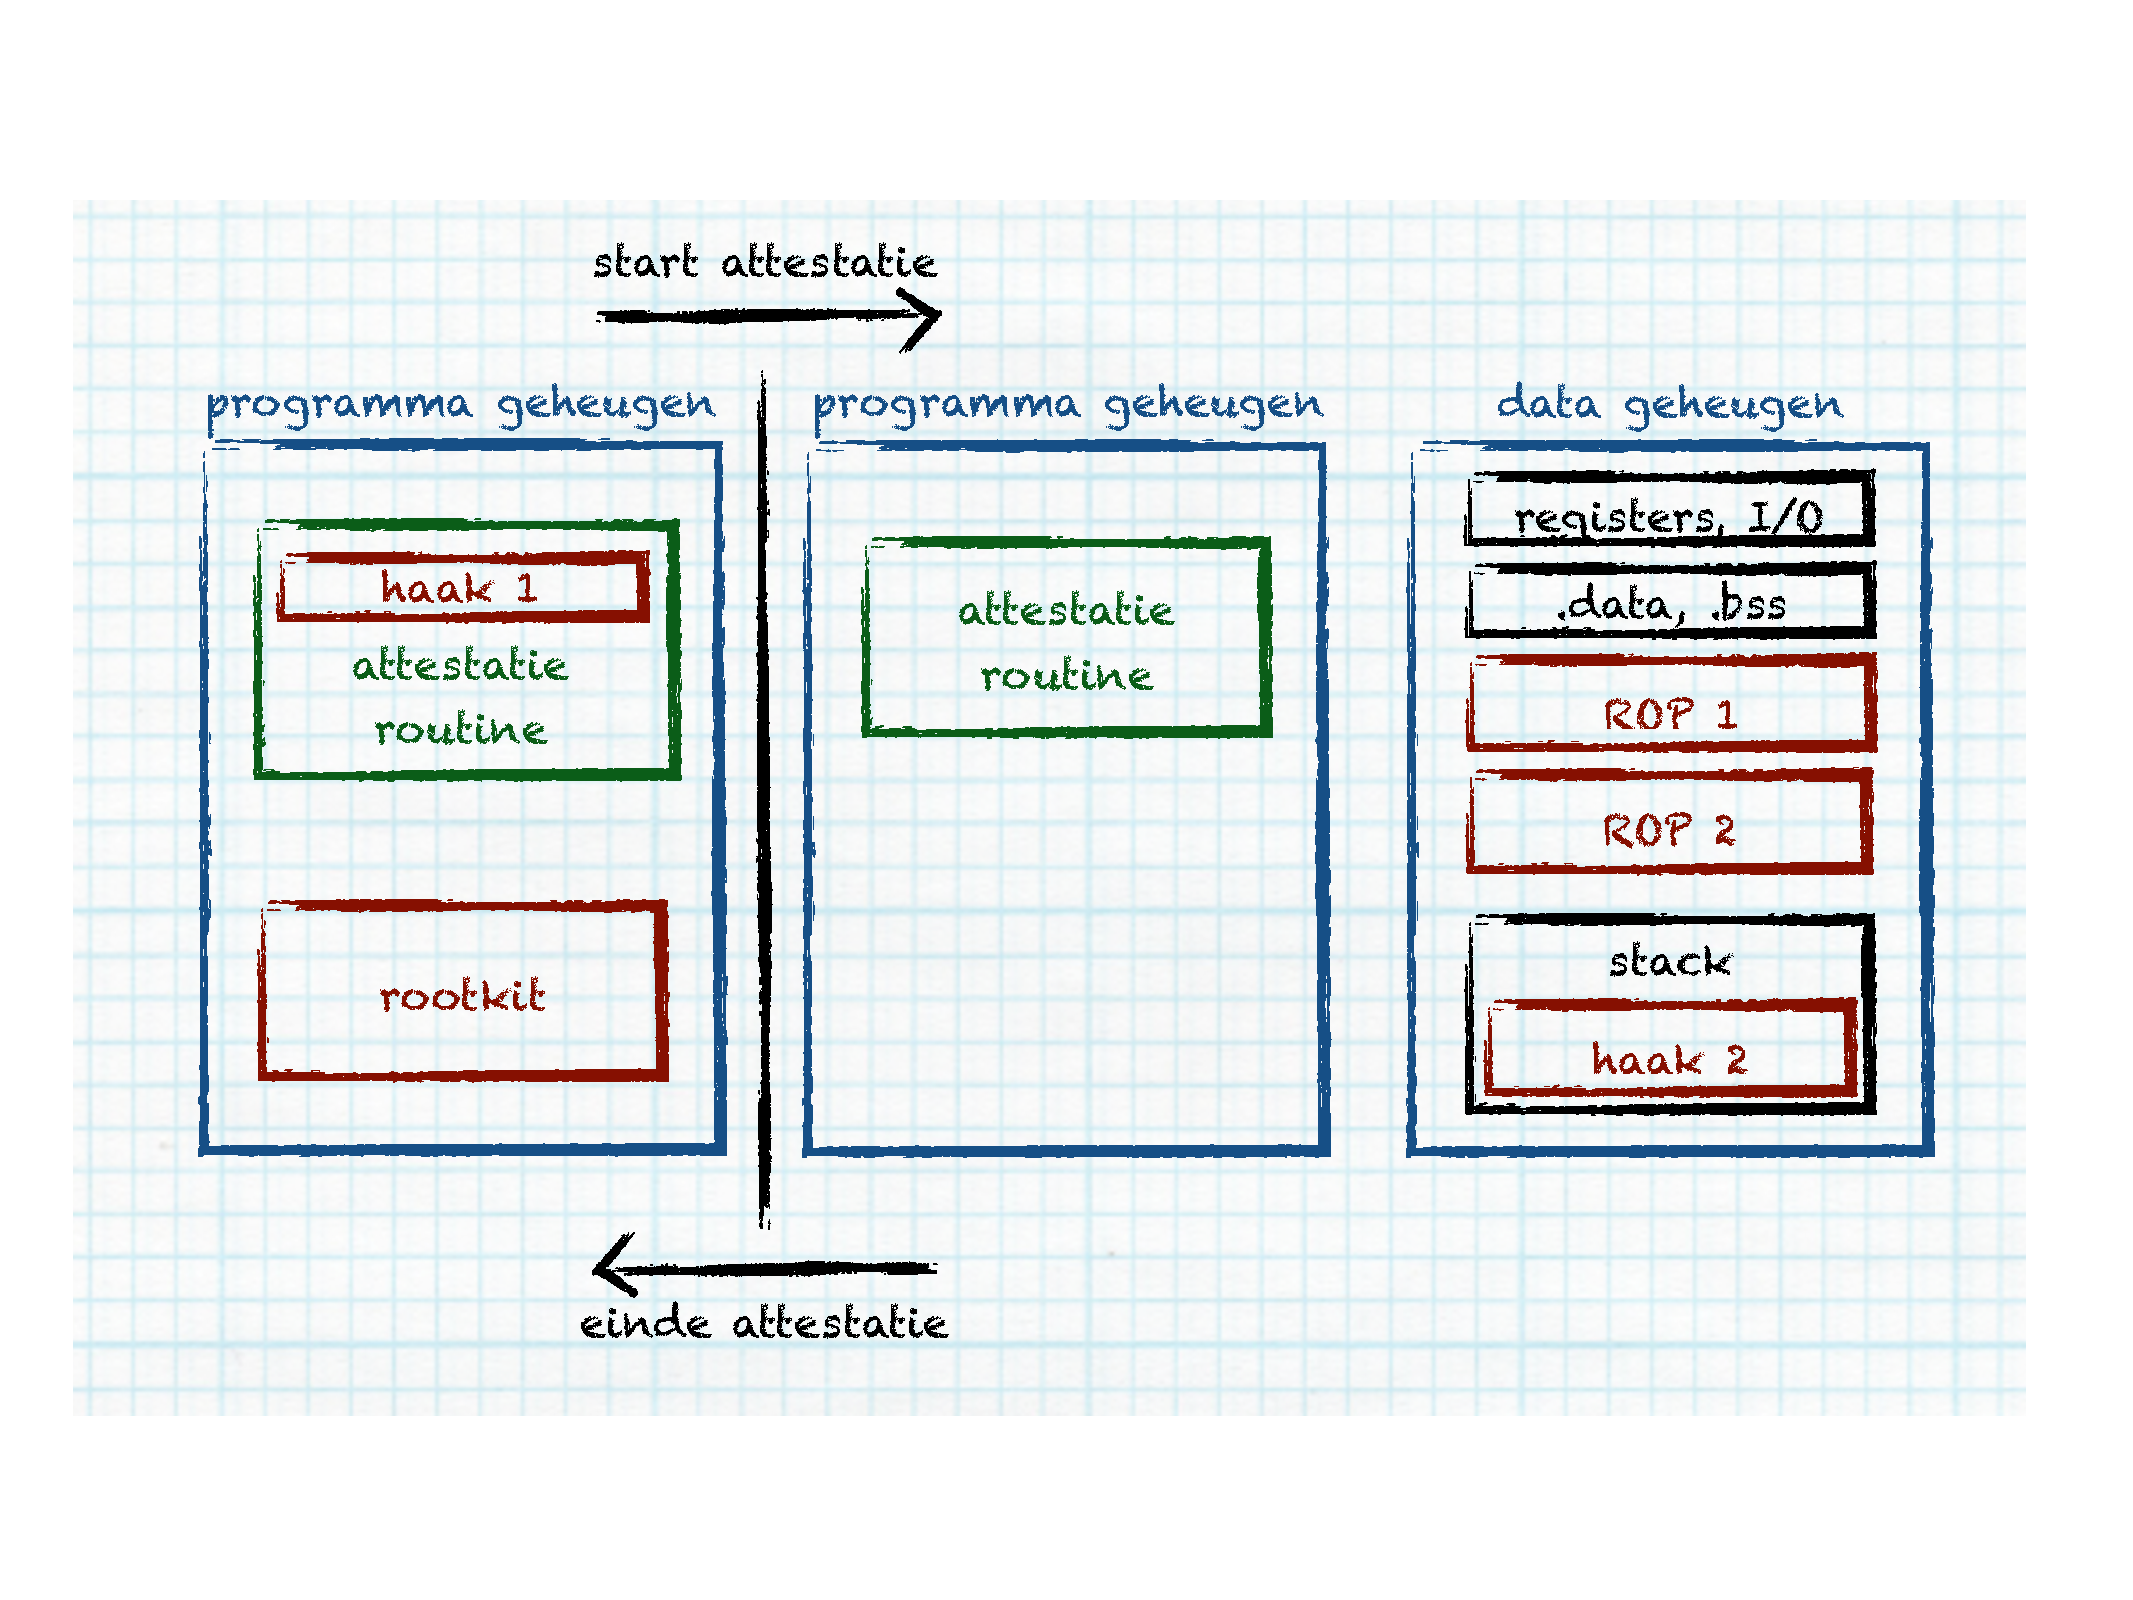
\includegraphics[width=0.9\linewidth]{resources/attestation-rootkit.pdf}
  \caption{De werking van een attestatie ontwijkende rootkit.}
  \label{fig:attestation-rootkit}
\end{figure}

Het verbergen van de rootkit en het herstellen van het programma geheugen in
zijn oorspronkelijke staat blijkt slechts een overhead van ongeveer 0.3\% op te
leveren t.o.v. bv. de SWATT attestatie techniek voorgesteld in
\cite{seshadri2004swatt}. Deze techniek controleert tevens de tijd dat de
attestatie routine nodig had om de checksum te berekenen. Indien deze te lang
duurt dan schrijft SWATT dit toe aan de overhead ge\"introduceerd door
mogelijke kwaadaardige code. Een verhoging met 0.3\% is mogelijk te weinig om
tot deze conclusie te komen.

Deze aanval richt zich nu louter op de attestatie routine, maar zoals in
\cite{perrig2010refutation} aangegeven wordt, it SWATT slechts een deel van een
volledige software attestatie en focust zich op het effectief attesteren van
code in het geheugen, niet op de omringende context. In een volledige
opstelling zou een attestatie procedure de het terugkeer adres op de stack mee
kunnen nemen in de attestatie.

\cite{castelluccia2009difficulty} beschrijven zelf enkele mogelijke pistes
waarmee een attestatie routine zichzelf zou kunnen beschermen tegen een
dergelijke rootkit. Een eerste zou op het einde van zijn implementatie het data
geheugen volledig leeg kunnen maken en vervolgens, zonder een terugkeer
operatie uit te voeren, waardoor de tweede haak vermeden wordt, de knoop te
herstarten. Het verwijderen van alle gegevens en het herstarten van een knoop
bij elk attestatie verzoek, kan afhankelijk van de functionaliteit die de knoop
aanbiedt, in de meeste gevallen niet wenselijk zijn. Dit euvel kan eventueel
wel ondervangen worden door het wegschrijven van deze gegevens naar een EEPROM.

Een andere oplossingsstrategie zou kunnen liggen in het attesteren van het data
geheugen. Dit moet dan wel op op het zelfde ogenblik gebeuren als de attestatie
van het programma geheugen, zodat de rootkit niet in staat is om zichzelf heen
en weer te kopi\"eren tussen de twee afzonderlijke attestaties. Zelfs al wordt
er willekeurig telkens uit het ene of het andere geheugen gelezen, dan nog kan
de rootkit zich nog steeds verplaatsen tussen de twee geheugens en moet deze
dat dan zelfs maar gemiddeld om de twee lees operaties doen. Hierdoor zal de
overhead zelfs gedeeld door twee worden, waardoor de impact ervan nog
moeilijker te detecteren wordt.

Tot slot is, zoals eerder reeds vermeld, het attesteren van het werkgeheugen op
zich reeds een zeer moeilijk gegeven, door de onvoorspelbare inhoud ervan.
Idealiter zou de vaststeller ook de inhoud van het volledige data geheugen
moeten kennen. Enerzijds bevat dit geheugen registers enz., welke volledig
onvoorspelbaar zijn en dus uitgesloten zouden moeten worden. Anderzijds bevat
het geheugen gegevens van de actieve processen. Deze zijn typisch afhankelijk
van opgemeten waarden en/of communicatie met andere knopen en dus per definitie
onvoorspelbaar voor de vaststeller.

Opnieuw zou het leegmaken van het data geheugen een voorspelbaar resultaat
opleveren voor de vaststeller, maar dit is dan evengoed een voorspelbaar
resultaat voor de aanvaller en kunnen opnieuw geheugen schaduwende technieken
gebruikt worden.

Naast SWATT werd in \cite{castelluccia2009difficulty} ook een
aanvalsmogelijkheid tegen ICE voorgesteld. Het \emph{checksum} algoritme van
ICE is zo geconstrueerd dat het niet mogelijk is om bij elke geheugentoegang na
te gaan of er een doorverwijzing moet gebeuren of niet. Maar het is wel
mogelijk om een consequentie bit-wijziging te doen, zonder voorafgaande test.

Algoritme \ref{alg:attestation-ice} toont het \emph{checksum} algoritme. De
eigenlijke berekening vanaf regel 4 bestaat uit een strikte afwisseling van
16 bit optellingen zonder overdracht en XOR operaties ($\oplus$).

\begin{algorithm}
\begin{algorithmic}[1]
  \Require{y, het aantal iteraties dat de verificatie routine uitvoert}
  \For{$l = y \: to \: 0$}
    \Let{$x$}{$x + (x^2 \vee 5) mod 2^{16}$} \Comment{T functie voor $0 < x < 2^{16}$}
    \Let{$daddr$}{$(daddr \oplus) \wedge MASK) + code\_start$} \Comment{adres gebaseerd op $x$.}
    \Let{$C_j$}{$C_j + PC$}   \Comment{Program Counter}
    \Let{$C_j$}{$C_j \oplus mem[daddr]$}  \Comment{het willekeurige geheugenadres}
    \Let{$C_j$}{$C_j + l$}
    \Let{$C_j$}{$C_j \oplus C_{j-1}$}
    \Let{$C_j$}{$C_j + x$}
    \Let{$C_j$}{$C_j \oplus daddr$}
    \Let{$C_j$}{$C_j + C_{j-2}$}
    \Let{$C_j$}{$C_j \oplus SR$}    \Comment{Status register}
    \Let{$C_j$}{\Call{rotate\_left}{$C_j$}}
    \Let{j}{$(j+1)\: mod \: 10$}
  \EndFor
\end{algorithmic}
\caption{ICE pseudo-code\label{alg:attestation-ice}}
\end{algorithm}

Een mogelijke aanval op ICE bestaat er in om twee wijzigingen aan te brengen
die elkaar opheffen, waardoor een zelfde checksum berekent wordt, maar er toch
iets anders berekend wordt. Praktisch is het mogelijk om de meest
betekenisvolle bit van de Program Counter en van de waarde van de opgehaalde
geheugenlocatie te wisselen. Door de opeenvolging van de optelling en de XOR
operatie zullen deze elkaar opheffen, zoals getoond wordt in de vergelijkingen
\ref{eq:attestation-ice} en \ref{eq:attestation-ice-bitflip}, waarin een
voorbeeld wordt gegeven met 8 bits argumenten.

\begin{equation} \label{eq:attestation-ice}
\begin{array}{cccccccccc}
       & c_{j-1}    & 1 &	0 &	1 &	0 &	1 &	1 &	1 &	0 \\
+	     & PC	        & 0	& 1	& 1	& 0	& 1	& 0	& 1	& 1 \\
\cline{1-10}
       &            &	0	& 0	& 0	& 1	& 1	& 0	& 0	& 1 \\
\oplus &	mem[addr]	& 0	& 1	& 1 &	0	& 1	& 1	& 0	& 1 \\
\cline{1-10}
       &            &	0	& 1	& 1	& 1	& 0	& 1	& 0	& 0 \\
\end{array}
\end{equation}

\begin{equation} \label{eq:attestation-ice-bitflip}
\begin{array}{cccccccccc}
       & c_{j-1}    & 1 &	0 &	1 &	0 &	1 &	1 &	1 &	0 \\
+	     & PC	        & \bm{1}	& 1	& 1	& 0	& 1	& 0	& 1	& 1 \\
\cline{1-10}
       &            &	\bm{1}	& 0	& 0	& 1	& 1	& 0	& 0	& 1 \\
\oplus &	mem[addr]	& \bm{1}	& 1	& 1 &	0	& 1	& 1	& 0	& 1 \\
\cline{1-10}
       &            &	0	& 1	& 1	& 1	& 0	& 1	& 0	& 0 \\
\end{array}
\end{equation}

Het resultaat van deze minimale aanpassingen is dat er zich een situatie
voordoet zoals weergegeven in figuur \ref{fig:attestation-ice-copy}, waarbij de
aanvaller zijn eigen aangepaste kopie van de ICE routine kan laten uitvoeren,
terwijl de geattesteerde regio zich elders bevindt, waardoor de routine niet
meer zelf-attesterend is en zijn beginsel verliest.

\begin{figure}
  \centering
  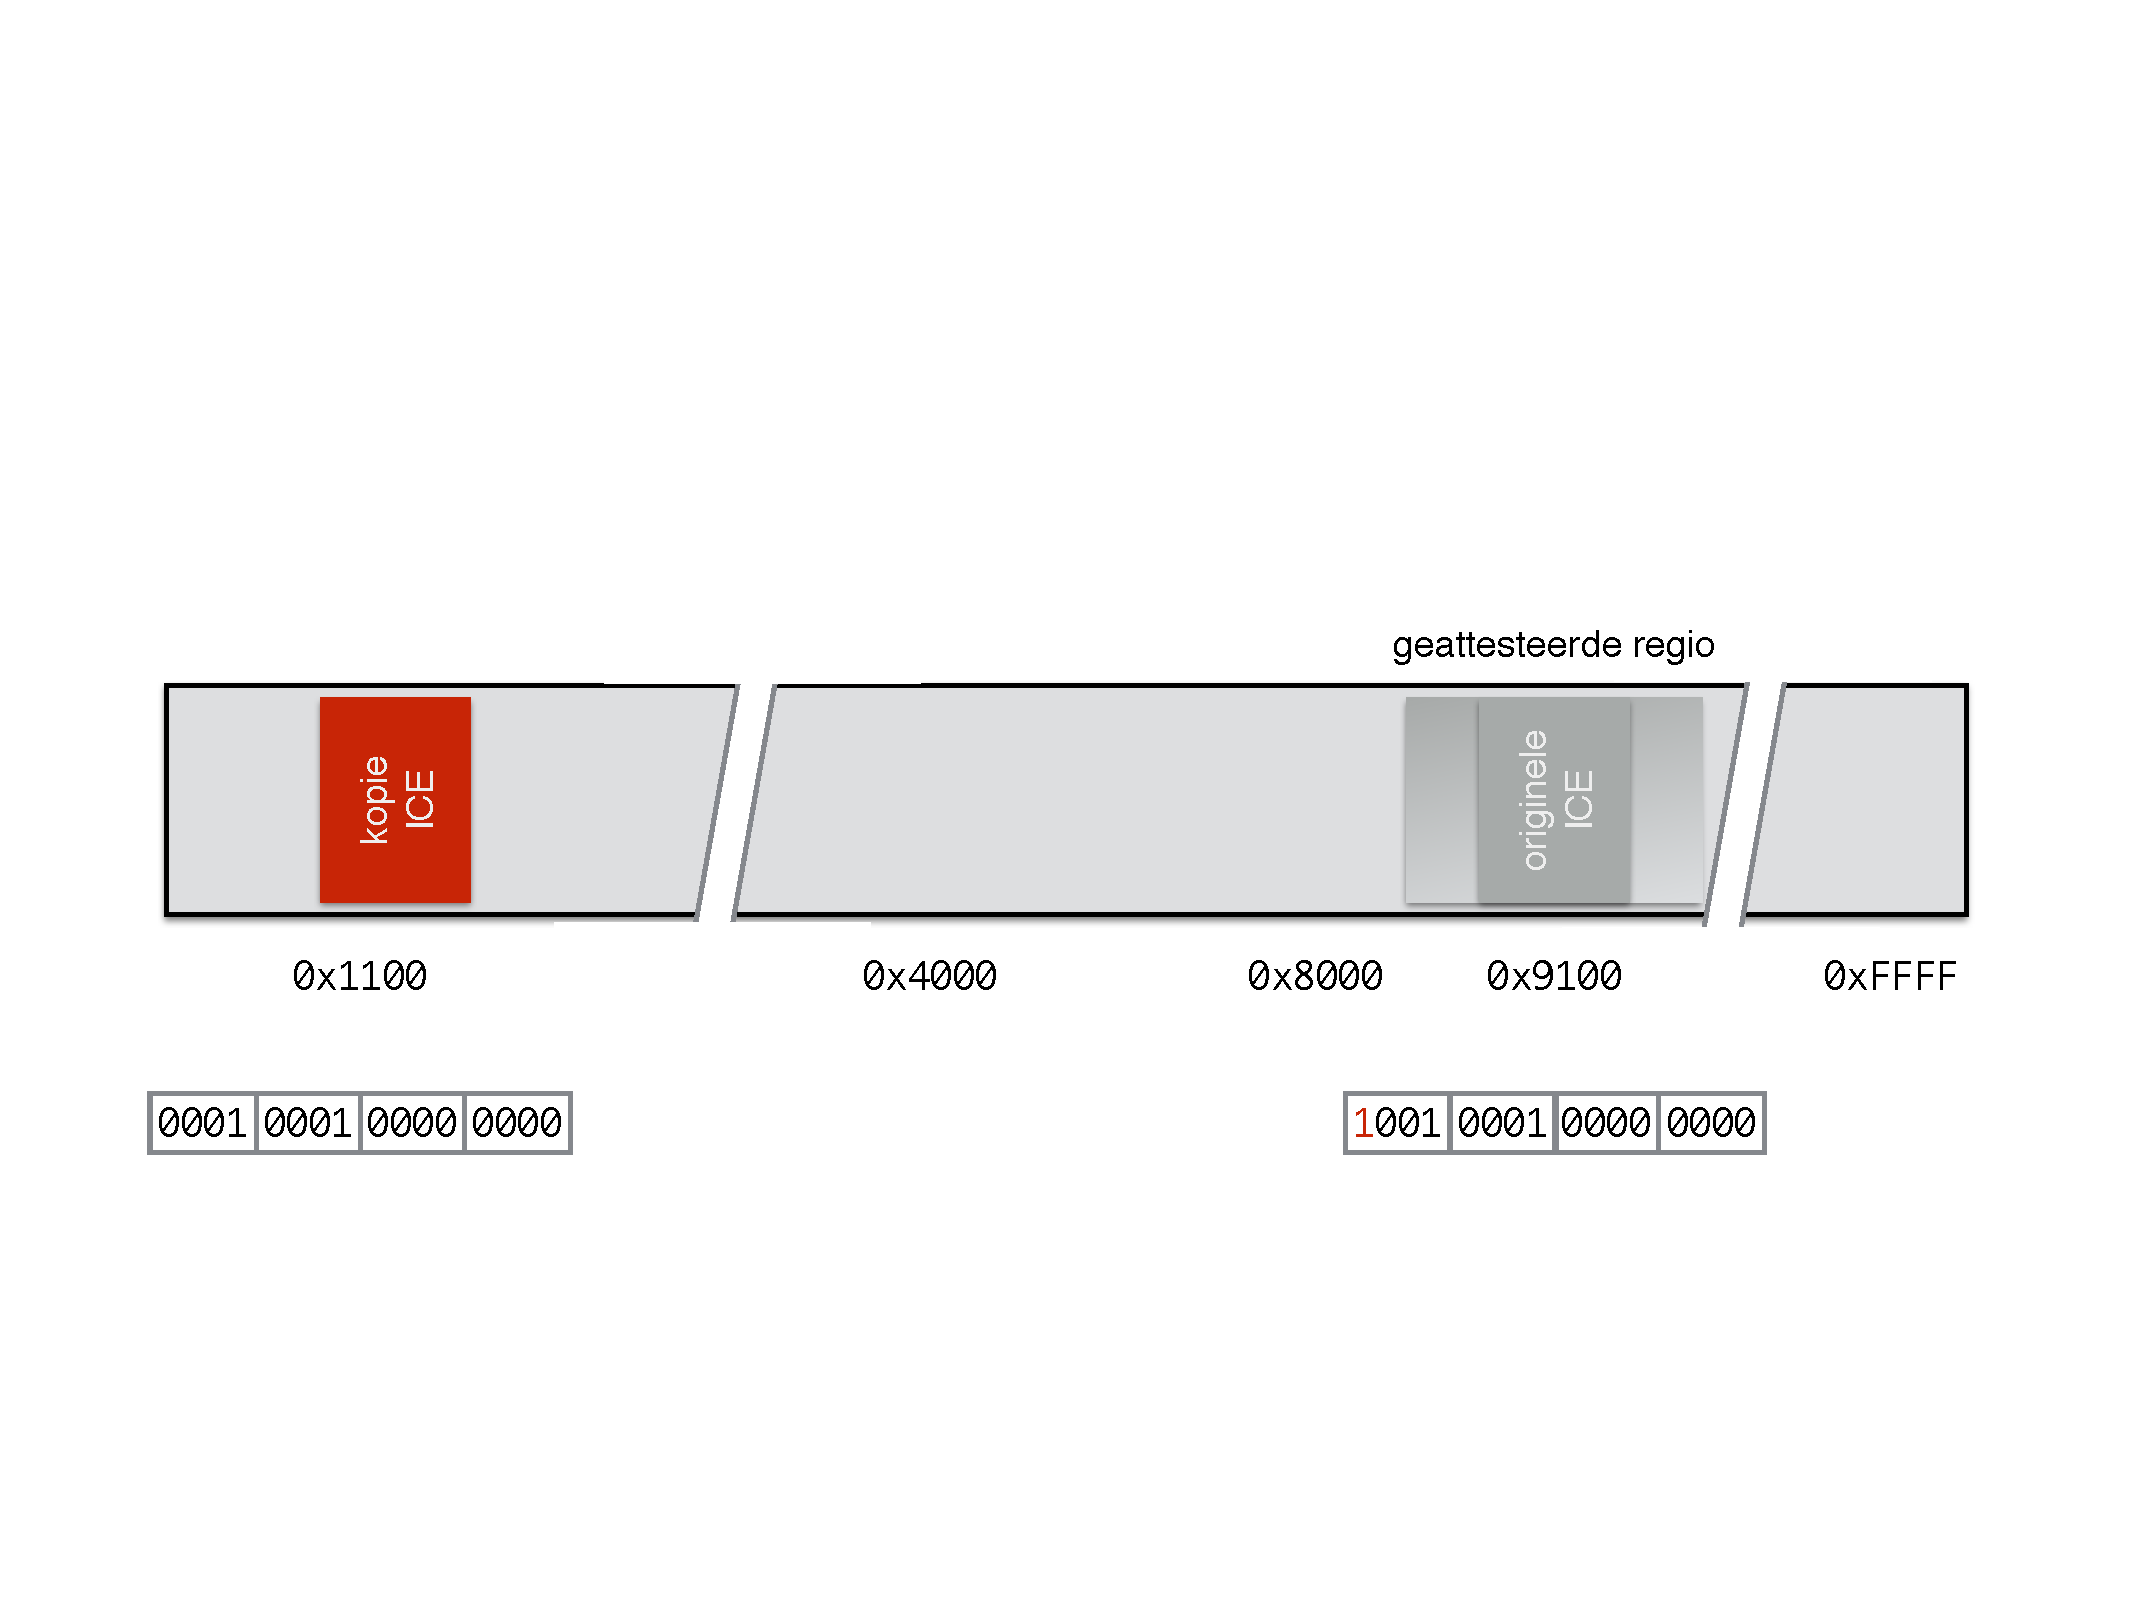
\includegraphics[width=0.9\linewidth]{resources/attestation-ice-copy.pdf}
  \caption{De legitieme ICE routine is opgeslagen op adres 0x9100 en een
  aangepaste kopie is opgeslagen op adres 0x1100. Deze twee adressen
  verschillen slechts in hun meest betekenisvolle bit. De aanvaller kan zijn
  aangepaste code gebruiken, maar nog steeds slagen voor de attestatie.}
  \label{fig:attestation-ice-copy}
\end{figure}

In \cite{perrig2010refutation} bevestigen de auteurs van ICE dat er fouten zijn
geslopen in de finale definitie van ICE en dat ze opportuniteiten hebben laten
liggen om deze aanval tegen te gaan.

\subsubsection*{Conclusies en gevolgen}

Uit voorgaande paragrafen kunnen we vaststellen dat het op een eenvoudige \mcu
zeer moeilijk maar mogelijk moet zijn om een sluitende oplossing voor software
attestatie uit te realiseren. Er zijn echter veel mogelijkheden waarbij de code
van een aanvaller zich steeds tussen de verschillende stappen in de attestatie
procedure kan wringen. Zelfs indien de vaststeller rekening houdt met de tijd
die de knoop nodig heeft om de attestatie te voltooien, zijn er technieken die
snel genoeg zijn om ook hier binnen de aannemelijke grenzen te vallen. Maar al
deze ingrepen zijn zeer complex en vragen een perfecte voorbereiding.

Aan de andere kant kan voor bijna elk van deze aanvallen wel een aanpassing
toegevoegd worden aan een bestaande attestatie, zodat de aanval verijdeld kan
worden. Zoals met veel jonge beveiligings-gerelateerde wetenschappen is ook
hier het kat en muis nog lang niet gedaan en is er nog ruimte voor verder
onderzoek.

We kunnen concluderen dat software attestatie op een eenvoudige \mcu mogelijk
is, maar met de nodige omzichtigheid moet ge\"implementeerd worden.

\subsubsection*{Trusted Platform Module - TPM}

In bovenstaande paragrafen, lag de nadruk op het software aspect van
attestatie. Voor \mcu's, met beperkte mogelijkheden, is het belangrijk om zo
effici\"nt mogelijk om te springen met energie. Maar ook de kostprijs is een
belangrijke factor, aangezien bijkomende kosten per knoop snel kunnen oplopen
in het kader van een volledig netwerk.

Software biedt in dit laatste geval dan logischerwijs een positief economisch
antwoord. Maar het is echter ook mogelijk om voor attestatie beroep te doen op
hardware. Daar waar een eenvoudige \mcu zich nagenoeg niet kan beschermen tegen
fysieke aanvallen, is het wel mogelijk om specifieke hardware te cre\"eren die
hermetisch afgesloten is.

Een voorbeeld hiervan is de \emph{Trusted Platform Module} of TPM, van de
\emph{Trusted Platform Group}. Dit is een specificatie op industrie-niveau die
toelaat om een vertrouwen te cre\"eren tussen verschillende ge\"informatiseerde
platformen in het algemeen. Deze specificatie is in 2009 ook opgenomen als een
ISO standaard\footnote{ISO/IEC 11889-1:2009 -
\url{http://www.iso.org/iso/catalogue_detail.htm?csnumber=50970}}.

In essentie is een TPM een smart-card die in staat is om cryptografische
gegevens op te slaan en bijhorende bewerking uit te voeren, zonder dat enige
interactie van de buitenwereld kan bewerkstelligd worden en het onmogelijk is
om de opgeslagen sleutels naar buiten te exporteren. Op deze manier kan de TPM
als een initi\"eel startpunt gebruikt worden om een keten van vertrouwen op te
bouwen.

Maar een extra TPM op een reeds beladen \mcu, is soms gewoon niet mogelijk.
Daarom stelt \cite{krauss2007detecting} voor om de mogelijkheden van een TPM op
de cluster hoofden (\ref{subsection:topology}), afgekort tot CH, binnen het
netwerk te gebruiken. Aangezien deze per definitie voorzien zijn om meer
energie te verbruiken, kan de bijkomende kost op dit niveau verantwoord worden.

Vanuit het oogpunt dat de werking van het netwerk moet gegarandeerd worden, kan
dit tevens een interessant gegeven zijn. Knopen, of cluster nodes (CN), die de
eigenlijke metingen doen en vervolgens doorsturen via een CH, kunnen nu deze
een verzoek tot attestatie sturen.

Deze functionaliteit wordt in een eerste protocol ge\"implementeerd als het
\emph{Periodic Broadcast Attestation Protocol}, of PBAP. De aanleiding van dit
protocol is terug te vinden in de manier waarop CNs communiceren met hun CH.
Indien elke CN individueel zijn CH zou gaan attesteren, zou dit een grote
overhead leggen op de CH. Door te opteren voor het periodiek uitsturen van
attestaties, kan de CH al zijn CNs in \'e\'en keer op de hoogte stellen. Het
feit dat CNs tussen twee metingen in slaap kunnen zijn, is inherent ondervangen
door het feit dat de CHs berichten voor hun CNs bufferen.

Deze attestatie focust zich op het garanderen dat de configuratie van het CH
ongewijzigd is sinds de installatie van het netwerk. Tijdens deze installatie
zal zo'n CH met zijn TPM een keten van hashes maken en deze blokkeren in de
TPM. Dit is een techniek die \emph{sealing}\footnote{Dit is slechts \'e\'en van
de basiscomponenten van een TPM. De volledige TPM functionaliteit wordt o.a. in
\cite{parno2010bootstrapping} toegelicht in het kader van de mogelijkheden die
een TPM biedt om als initi\"ele bron van vertrouwen gebruikt te worden.}
genoemd wordt. De TPM zal deze hashes alleen vrijgeven indien deze de
configuratie van de CH kan valideren als ongewijzigd.

Door de laatste hash uit de keten van elke CH te verdelen over de CNs, wordt
het voor hen opnieuw mogelijk om boodschappen van de CH te valideren. We nemen
aan dat het CH en de CNs lichtelijk gesynchroniseerd zijn qua tijd en dat zij
de evolutie van de tijd onderling herkennen als intervallen die aangeduid wordt
met $I_\lambda$.

Indien $CH_i$ op ogenblik $I_\lambda$ inderdaad nog steeds dezelfde
configuratie heeft als initieel, zal de TPM de volgende hash uit de keten
vrijgeven: $c_{n-\lambda}^{CH_i}$\footnote{De keten was gebaseerd op de
init\"ele hash $c_0^{CH_i}$ en werd opgebouwd tot $c_n^{CH_i}$, welke
vrijgegeven werd aan de verschillende CNs.}.

De CH kan deze nieuw vrijgegeven hash nu distribueren naar de CNs, welke deze
kunnen valideren aan de hand van de vorig gekende hash:
$H(c_{n-\lambda}^{CH_i}) \overset{?}{=} c_{n-\lambda+1}^{CH_i}$. Aangezien de
CH slechts over deze hash kan beschikking indien deze is vrijgegeven door de
TPM en aangezien dit slechts gebeurd wanneer de systeem configuratie van de CH
niet gewijzigd is, heeft de CN een garantie dat de CH ongewijzigd en
betrouwbaar is.

Maar ook individuele attestaties zijn mogelijk, in de vorm van het
\emph{Individual Attestation Protocol} of IAP. Hierbij wordt er een
symmetrische encryptie sleutel $K_{CN_j,CH_i}$ gegenereerd en opgeslagen in de
TPM. De CH zal deze sleutel alleen kunnen gebruiken vanuit zijn TPM en deze zal
er slechts toegang toe verschaffen indien de configuratie van de CH ongewijzigd
is.

Een CN die nu zijn CH wil attesteren, kan nu een eenmalig en uniek getal, of
\emph{nonce}, samen mijn zijn unieke identificatie ($ID_{CN_j}$) versleutelen
en naar zijn CH sturen. Indien deze over een ongewijzigde configuratie
beschikt, zal de TPM hem toelaten om de versleutelde boodschap te decoderen en
de oorsprong van de boodschap te valideren aan de hand van $ID_{CN_j}$. De CH
kan vervolgens de \emph{nonce} opnieuw versleutelen en terug sturen naar de CN.
Deze kan tot slotte opnieuw deze boodschap decoderen en vaststellen of de CH
inderdaad dezelfde \emph{nonce} terug stuurde. Omdat de CN weet dat de CH
slechts over $K_{CN_j,CH_i}$ kan beschikken indien zijn configuratie
ongewijzigd is, beschikt de CN over voldoende aanwijzing dat de CH betrouwbaar
is.

\subsubsection*{Gedistribueerde attestatie}

In \ref{subsection:cooperation} zagen we reeds een implementatie van het Guy
Fawkes protocol, waardoor een groep van knopen toch een stemming konden houden
in het bijzijn van veroverde knopen. Een andere voorbeeld van een co\"operatief
algoritme binnen de context van software attestatie wordt voorgesteld in
\cite{yang2007distributed}. Om te vermijden dat aanvallers het lege programma
geheugen gebruiken om een kopie van de originele software van een knoop op te
slaan, wordt voordat een knoop in gebruik wordt genomen, deze lege ruimte
opgevuld met pseudo-willekeurige getallen. Dit gebeurt voor knoop $u$ op basis
van een initi\"ele waarde $S_u$, de zgn. \emph{seed}

Als knoop $u$ $n$ buren heeft, kiest $u$ $k - 1$ ($1 \leq k \leq n$)
willekeurige constante termen $a_1, a_2, \dots a_{k-1}$ uit een eindig
priemveld $Z_p$. Hiermee wordt de functie $f(x) = S_u + a_1 x+a_2 x^2 + \dots +
a_{k-1} x^{k-1}$, waarvoor evident $f(0) = S_u$. Vervolgens berekent en
verdeeld de knoop koppels van de vorm $(i,f(i))$ onder zijn buren en verwijdert
uiteindelijk $S_u$ uit zijn geheugen.

Op dit ogenblik beschikt geen enkele individuele knoop over de sleutel om de
pseudo-willekeurige inhoud van knoop $u$ opnieuw te berekenen, zelfs knoop $u$
zelf niet. Deze heeft alleen het resultaat in het geheugen staan.

De attestatie van knoop $u$ gebeurt dan als volgt: alle buren selecteren
\'e\'en knoop uit hun groep en sturen elk hun waarde $f(i)$ naar deze knoop. Op
basis van deze waarden kan via Lagrange interpolatie de functie terug opgesteld
worden en kan $S_u = f(0)$ berekend worden door deze knoop. Vervolgens kan deze
knoop knoop $u$ attesteren door het sturen van een challenge en kan deze
valideren door zelf ook deze berekening te maken.

De techniek is zonder meer interessant, maar is onderhevig aan verschillende
problemen. Zo kan een aanvaller trachten een geselecteerde knoop onder controle
te krijgen, waardoor hij in staat is om diens opnieuw samengestelde initi\"ele
waarde te bemachtigen. Nadien is hij in staat om die zelfde knoop te veroveren
en te voorzien van code die gebruik maakt van de veroverde initi\"ele waarde om
de pseudo-willekeurige getallen te generen en de lege ruimte opnieuw te
gebruiken voor zijn eigen doeleinden.

De auteurs beseffen dit probleem ook en stellen daarom een aangepast algoritme
voor, dat tevens de herberekening van de \emph{checksums} door de attesterende
buren vermijdt.

In plaats van de koppels $(i, f(i))$ te versturen naar alle buren, verstuurt de
knoop nu koppels die bestaan uit een challenge en een berekende \emph{checksum}
voor die challenge: $(C_i,R_i)$. Deze worden verdeeld onder de buren, die nu
elk \'e\'en valide combinatie hebben.

Wanneer een knoop nu geattesteerd wordt, zal elk van de buren om de beurt een
challenge aanbieden aan de knoop. Hierna volgt een stem-ronde op basis van de
antwoorden.

De complexiteit van deze strategie is veel hoger voor een aanvaller. Geen
enkele knoop beschikt nu nog over de initi\"ele waarde $S_u$, zelfs niet
tijdelijk om de validatie te doen. De gedistribueerde validatie berust op
evenveel unieke controles als er buren zijn. Dit zou de aanvaller verplichten
om de challenge/response koppels bij elk van de buren te veroveren om zo
\'e\'en knoop te kunnen voorzien van code die een attestatie zou kunnen
weerstaan.

\subsubsection*{Case Study: Slimme meters}

-> AMI situatie \cite{lemay2012cumulative}

\TODO

%!TEX root=masterproef.tex

\subsection{Raamwerken voor detectie}
\label{subsection:frameworks}

Naast het onderzoek naar de verschillende autonome detectiealgoritmen, zijn er
ook onderzoekers actief op zoek naar manieren om meer holistische oplossingen
te bouwen die eerder het probleem als een geheel beschouwen in plaats van de
som van kleine, losse delen. In deze sectie bekijken we een aantal van deze
voorgestelde raamwerken.

\subsubsection*{Di-Sec}
\label{subsubsection:di-sec}

In \citep{valero2012di} komen de auteurs tot dezelfde conclusie als wat wij
hier enkele malen hebben aangehaald: er wordt veel gekeken naar
detailoplossingen, maar zelden wordt een algemene oplossing voorgesteld voor de
typische situatie van WSN. De auteurs zijn het verder ook eens met de stelling
dat het belangrijk is om te leren van deze detailoplossingen, om een eventueel
raamwerk af te stemmen op deze oplossingen, en gebruik te maken van de goede
eigenschappen ervan, bij de implementatie van het eigenlijke raamwerk.

De auteurs gaan er in hun redenering van uit dat, gegeven de eigenheid van het
draadloze medium, veel aanvallen zich richten op deze communicatievorm. Ze
defini\"eren daarom een eerste component, \ttt{COMM}, die zich toespitst op
communicatie en waarlangs alle gegevens passeren die verstuurd en/of ontvangen
worden. Daarnaast zijn er nog drie bijkomende componenten: \ttt{M-Core}, de
centrale controlemodule, \ttt{Sense}, de sensormodule en de \ttt{DDMs}, de
detectie- en verdedigingsmodules. Deze laatste zijn aanvalspecifieke modules
die ingevoegd kunnen worden in het raamwerk. Figuur
\ref{fig:di-sec-architecture} geeft een overzicht van de architectuur voor het
raamwerk, genaamd Di-Sec.

\begin{figure}[ht]
  \centering
  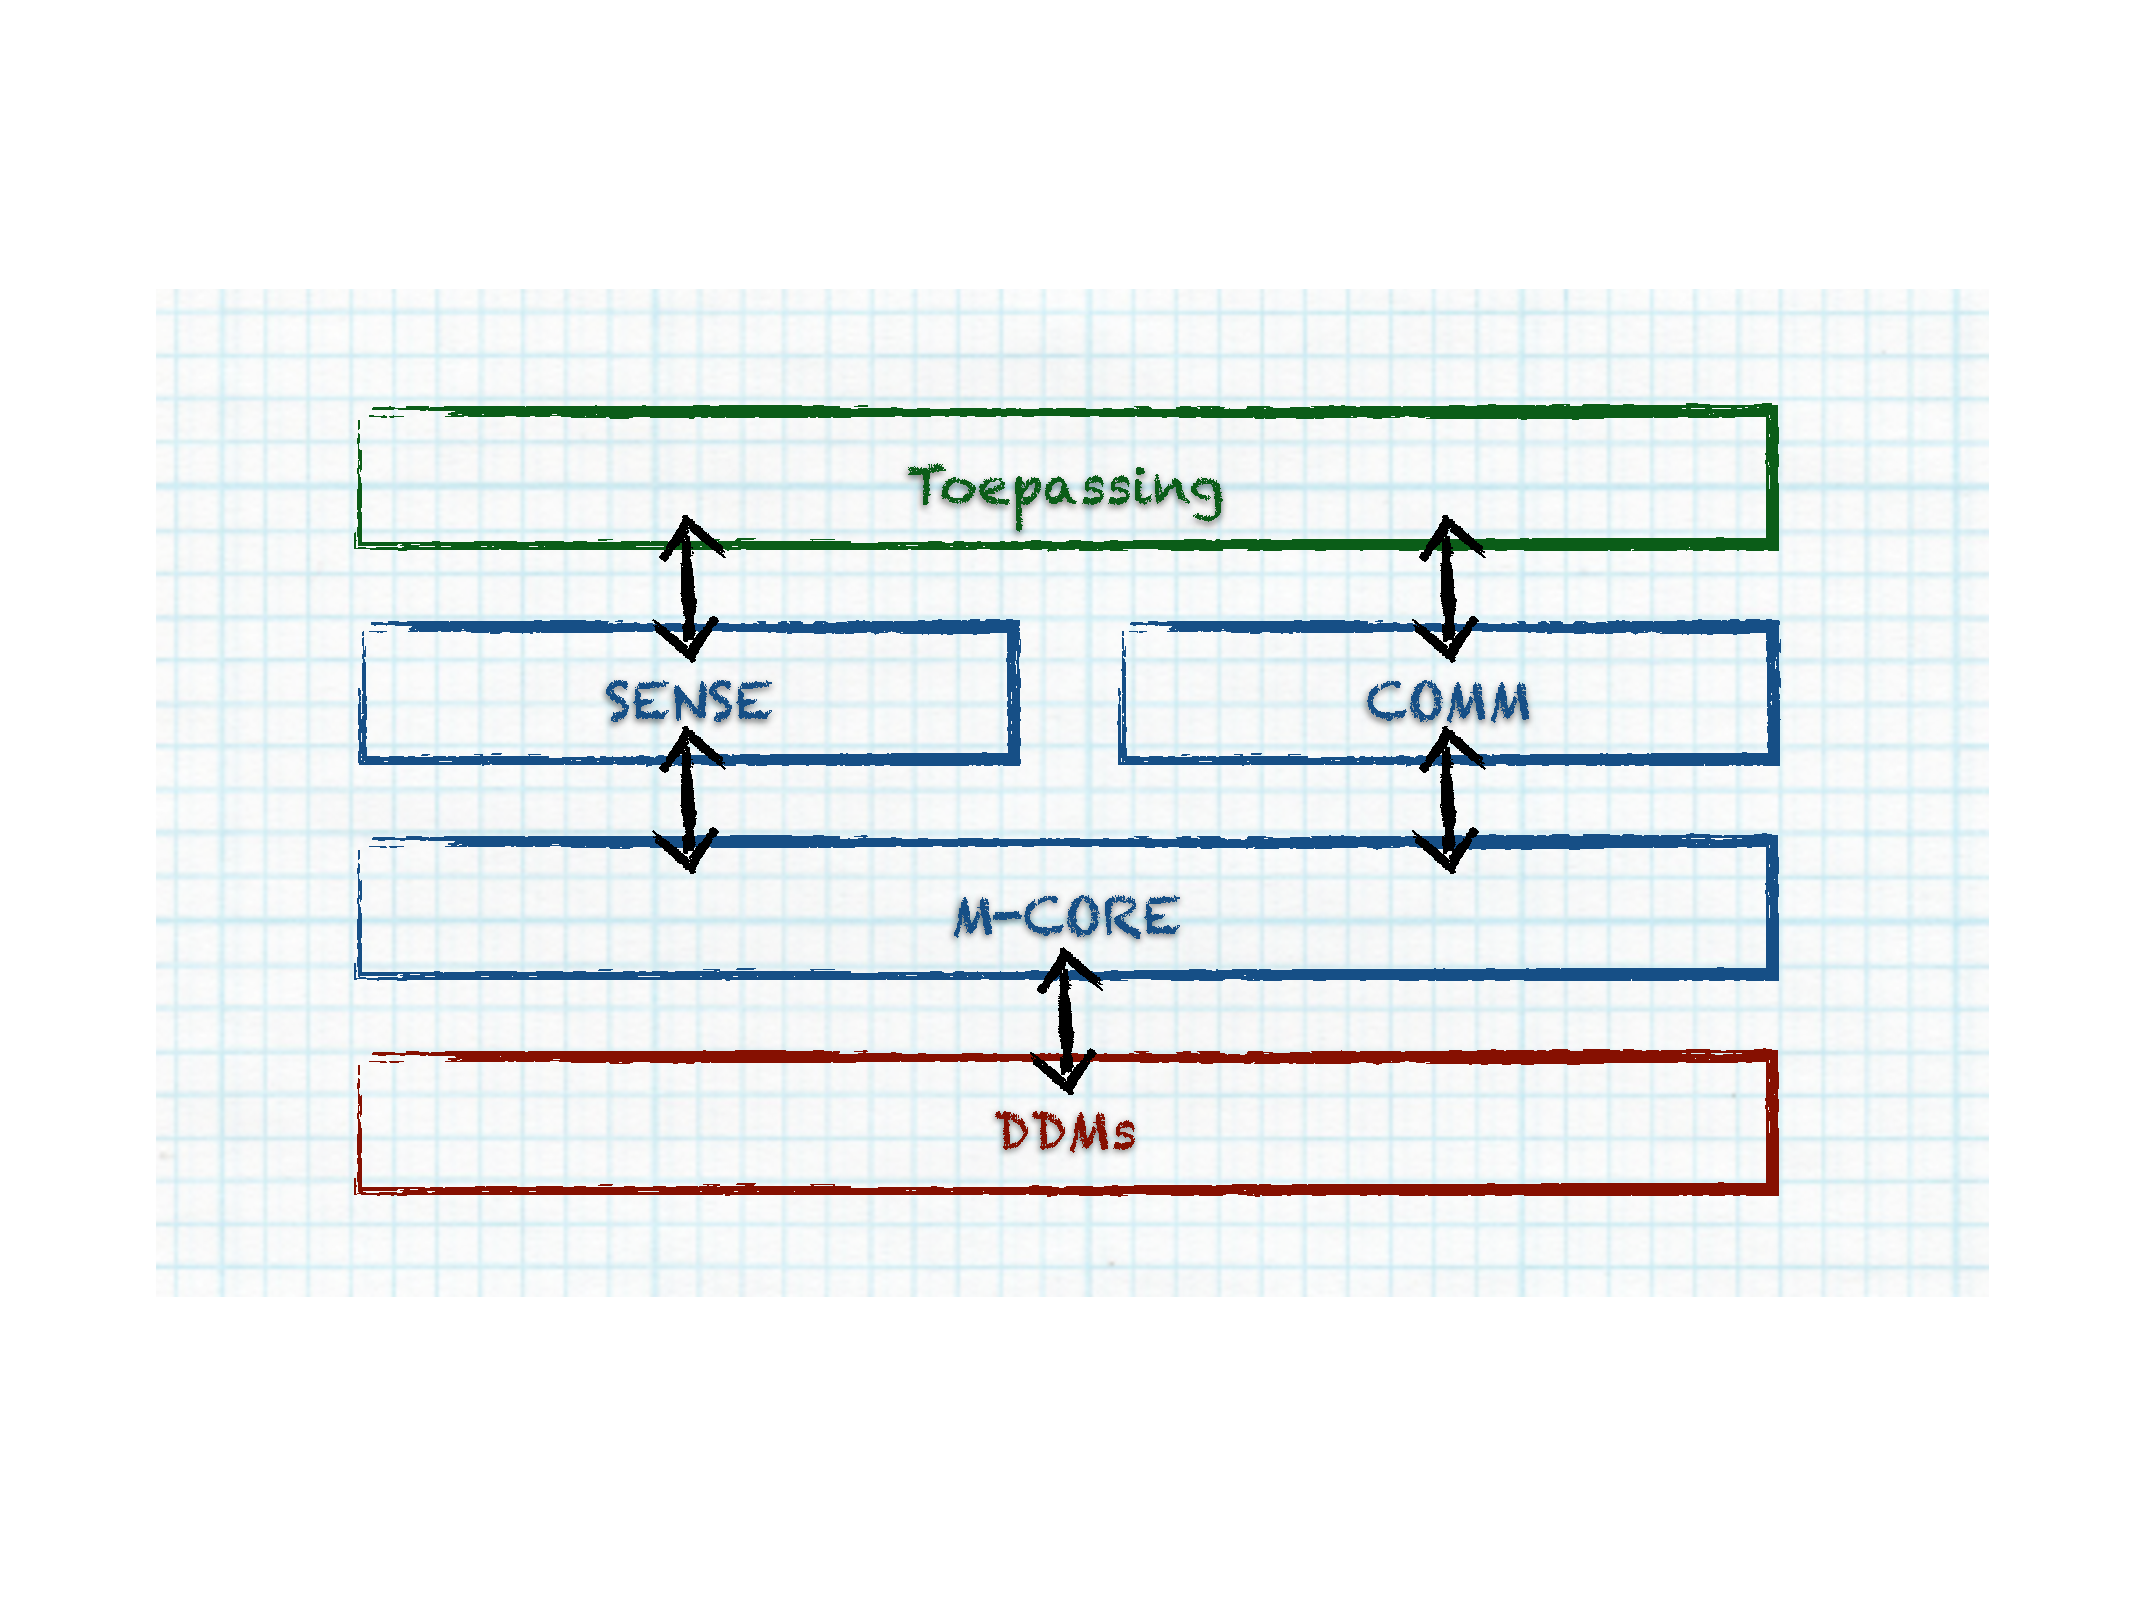
\includegraphics[width=0.8\linewidth]{resources/di-sec-architecture.pdf}
  \caption[Architectuur van Di-Sec]{Architectuur van Di-Sec (Bron:\citep{valero2012di})}
  \label{fig:di-sec-architecture}
\end{figure}

De drie modules vormen als het ware een API voor de \ttt{DDMs}. De manier
waarop \ttt{COMM} en \ttt{Sense} de toegang tot alle in- en uitvoer, zowel de
netwerkcommunicatie als de toegang tot de sensoren, hermetisch afsluiten, toont
aan dat Di-Sec een raamwerk is voor het ontwikkelen van sensorknopen.

Naast dit raamwerk, biedt Di-Sec ook een eigen taal aan om Di-Sec te gebruiken:
de \ttt{M-Core} controle taal (MCL). Deze laat toe om met een beperkte taal de
nodige sjablonen te maken waarmee nieuwe modules ontwikkeld kunnen worden en
alsook om de nodige aanpassingen te doen aan de configuratiebestanden.

\subsubsection*{Architectuur voor een sensorknoop}
\label{subsubsection:node-architecture}

Daar waar Di-Sec zich vooral focust op het aanbieden van een API voor het
ontwikkelen van detectiemodules, gaat \citep{zhang2000intrusion} een stap
verder en verrijkt de architectuur van een sensorknoop met verschillende
modules, gericht op de onderliggende processen van een IDS. Zo worden
beveiligde communicatiemodules voorzien, is er een co\"operatieve
detectiemodule, en voorzien zij globaal aggregerende modules om tot een
consensus te komen op het niveau van het netwerk. Deze architectuur is
schematisch weergegeven in figuur \ref{fig:node-architecture}.

\begin{figure}[ht]
  \centering
  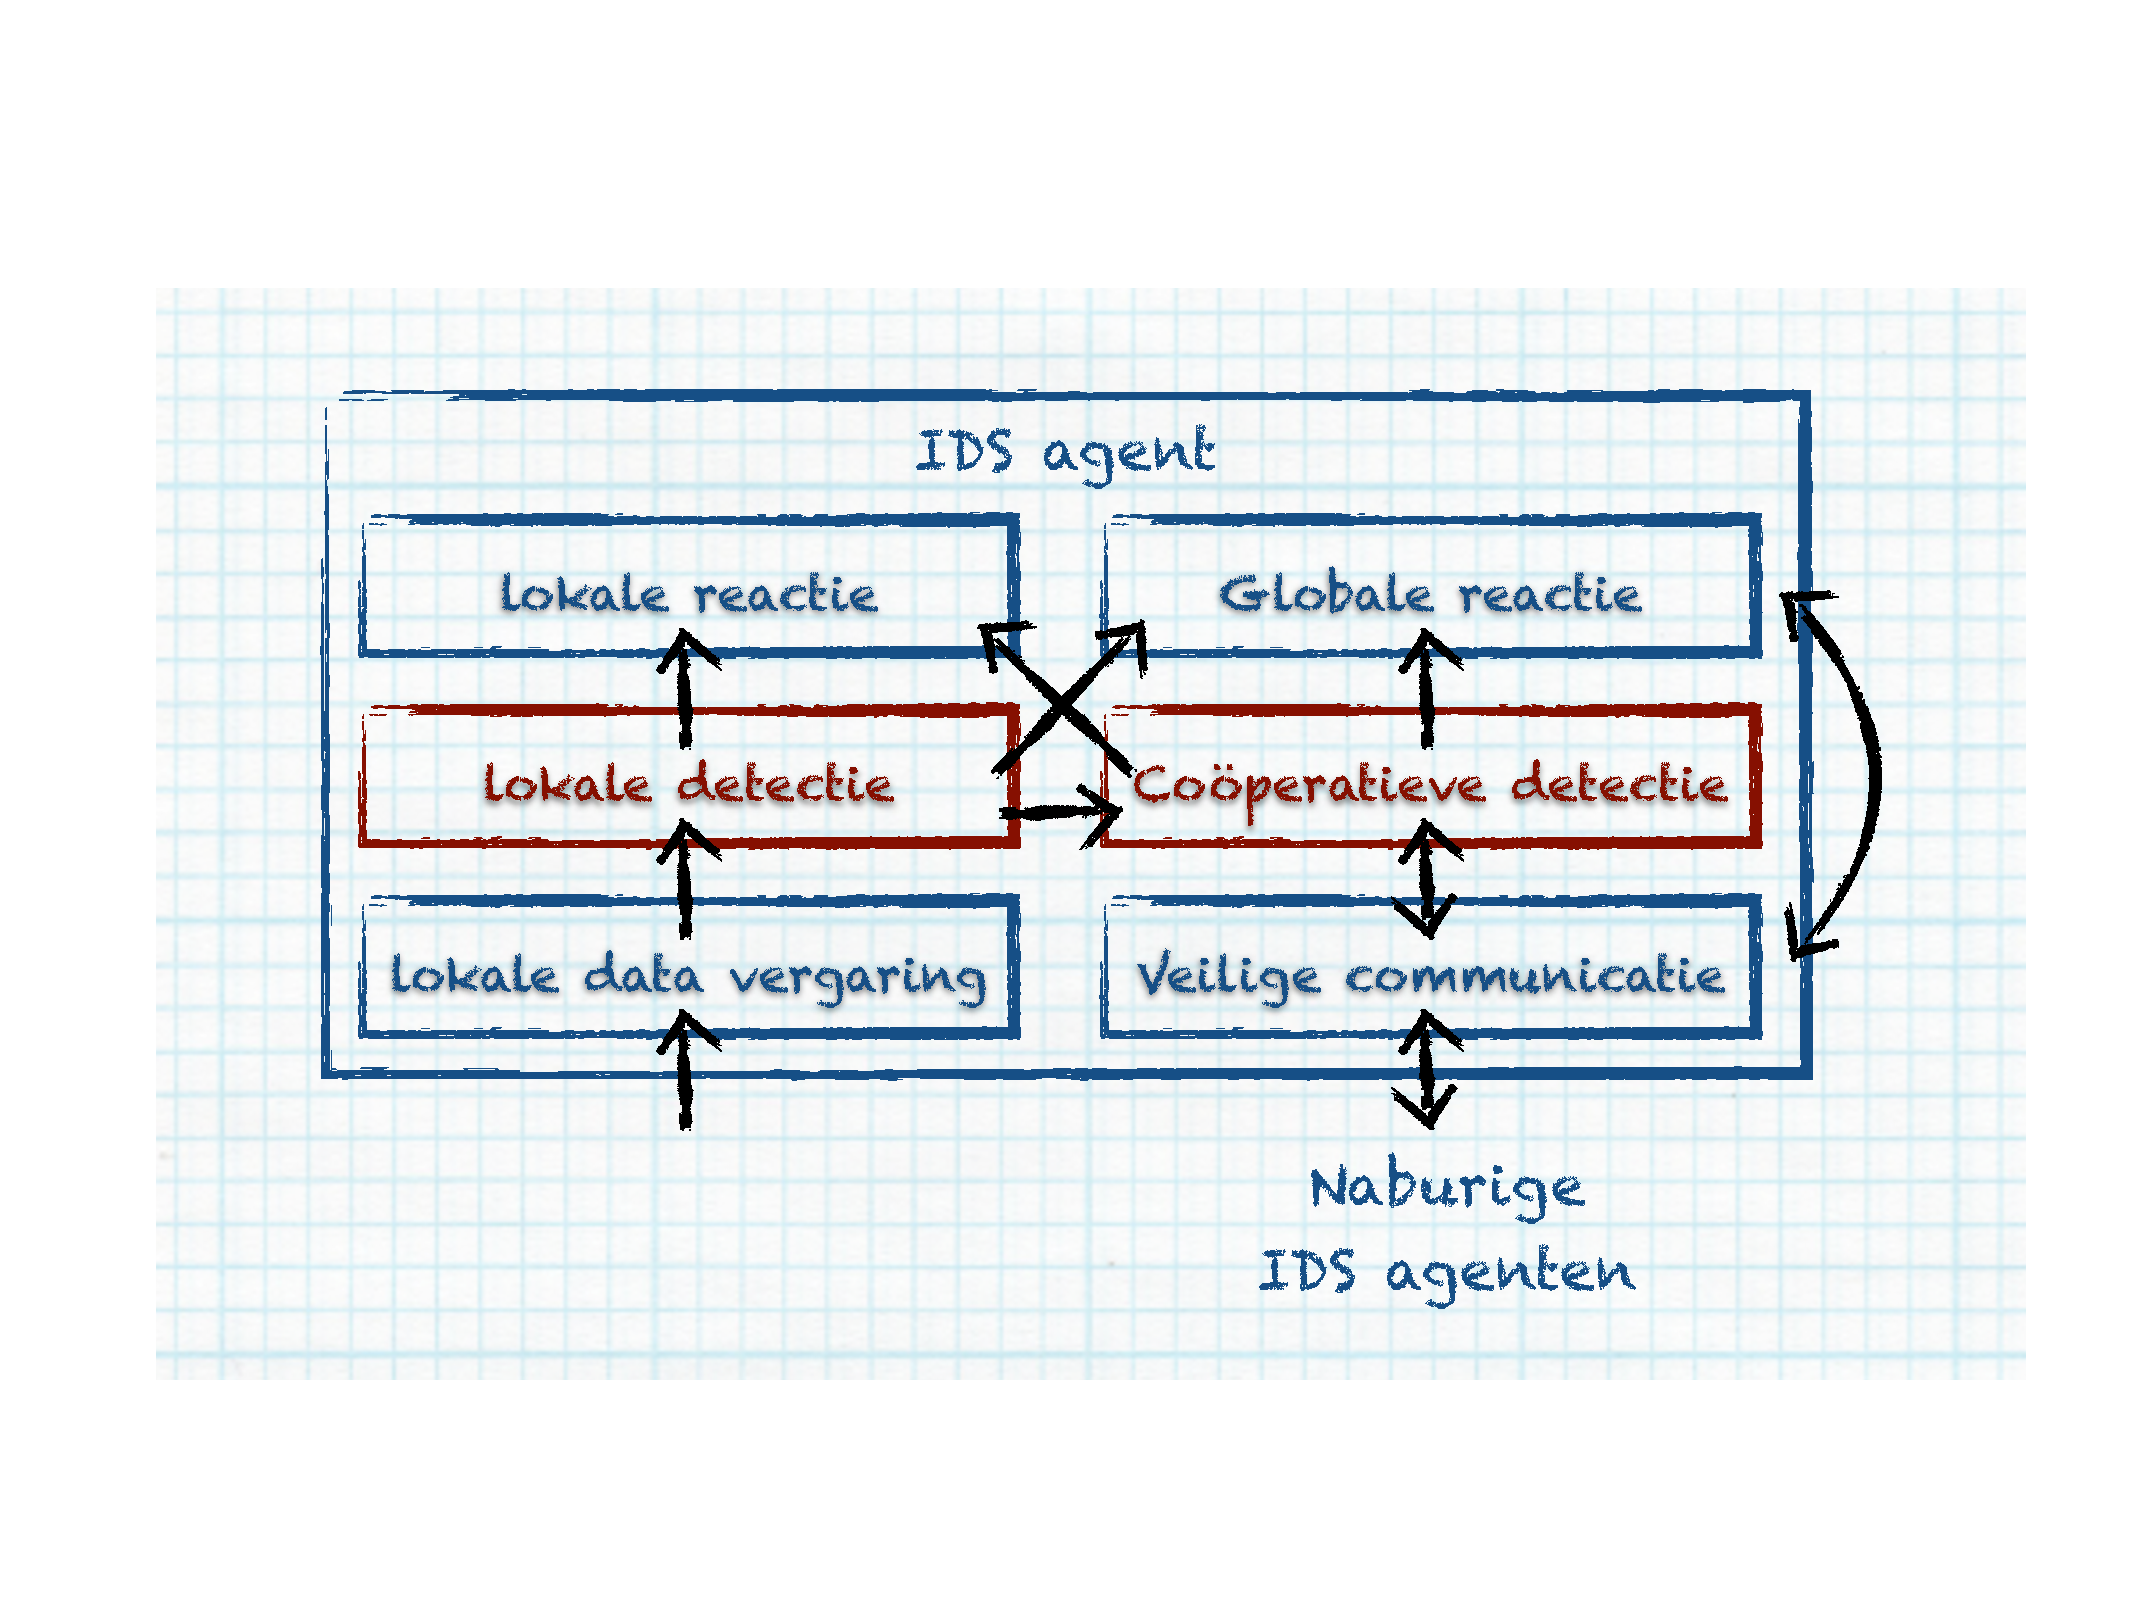
\includegraphics[width=0.9\linewidth]{resources/node-architecture.pdf}
  \caption[Model voor een IDS op een sensorknoop]{Model voor een IDS op een
  sensorknoop (Bron:\citep{zhang2000intrusion})}
  \label{fig:node-architecture}
\end{figure}

De co\"operatieve modules voorzien bv. mogelijkheden om zekerheden te koppelen
aan beweringen over bepaalde gebeurtenissen. Op deze manier biedt de
architectuur een zeer specifiek aanbod aan functionaliteit, specifiek voor het
bouwen van een IDS.

Een gelijkaardige architectuur wordt voorgesteld in \citep{krontiris2008lidea}.
LIDeA is een uitgewerkte architectuur voor de idee\"en die al aan bod kwamen in
sectie \ref{subsection:cooperation}. Ze vormen het platform waarop het
co\"operatieve algoritme van \citep{krontiris2009cooperative} ge\"ent is.
Figuur \ref{fig:lidea-architecture} toont de LIDeA architectuur.

\begin{figure}[ht]
  \centering
  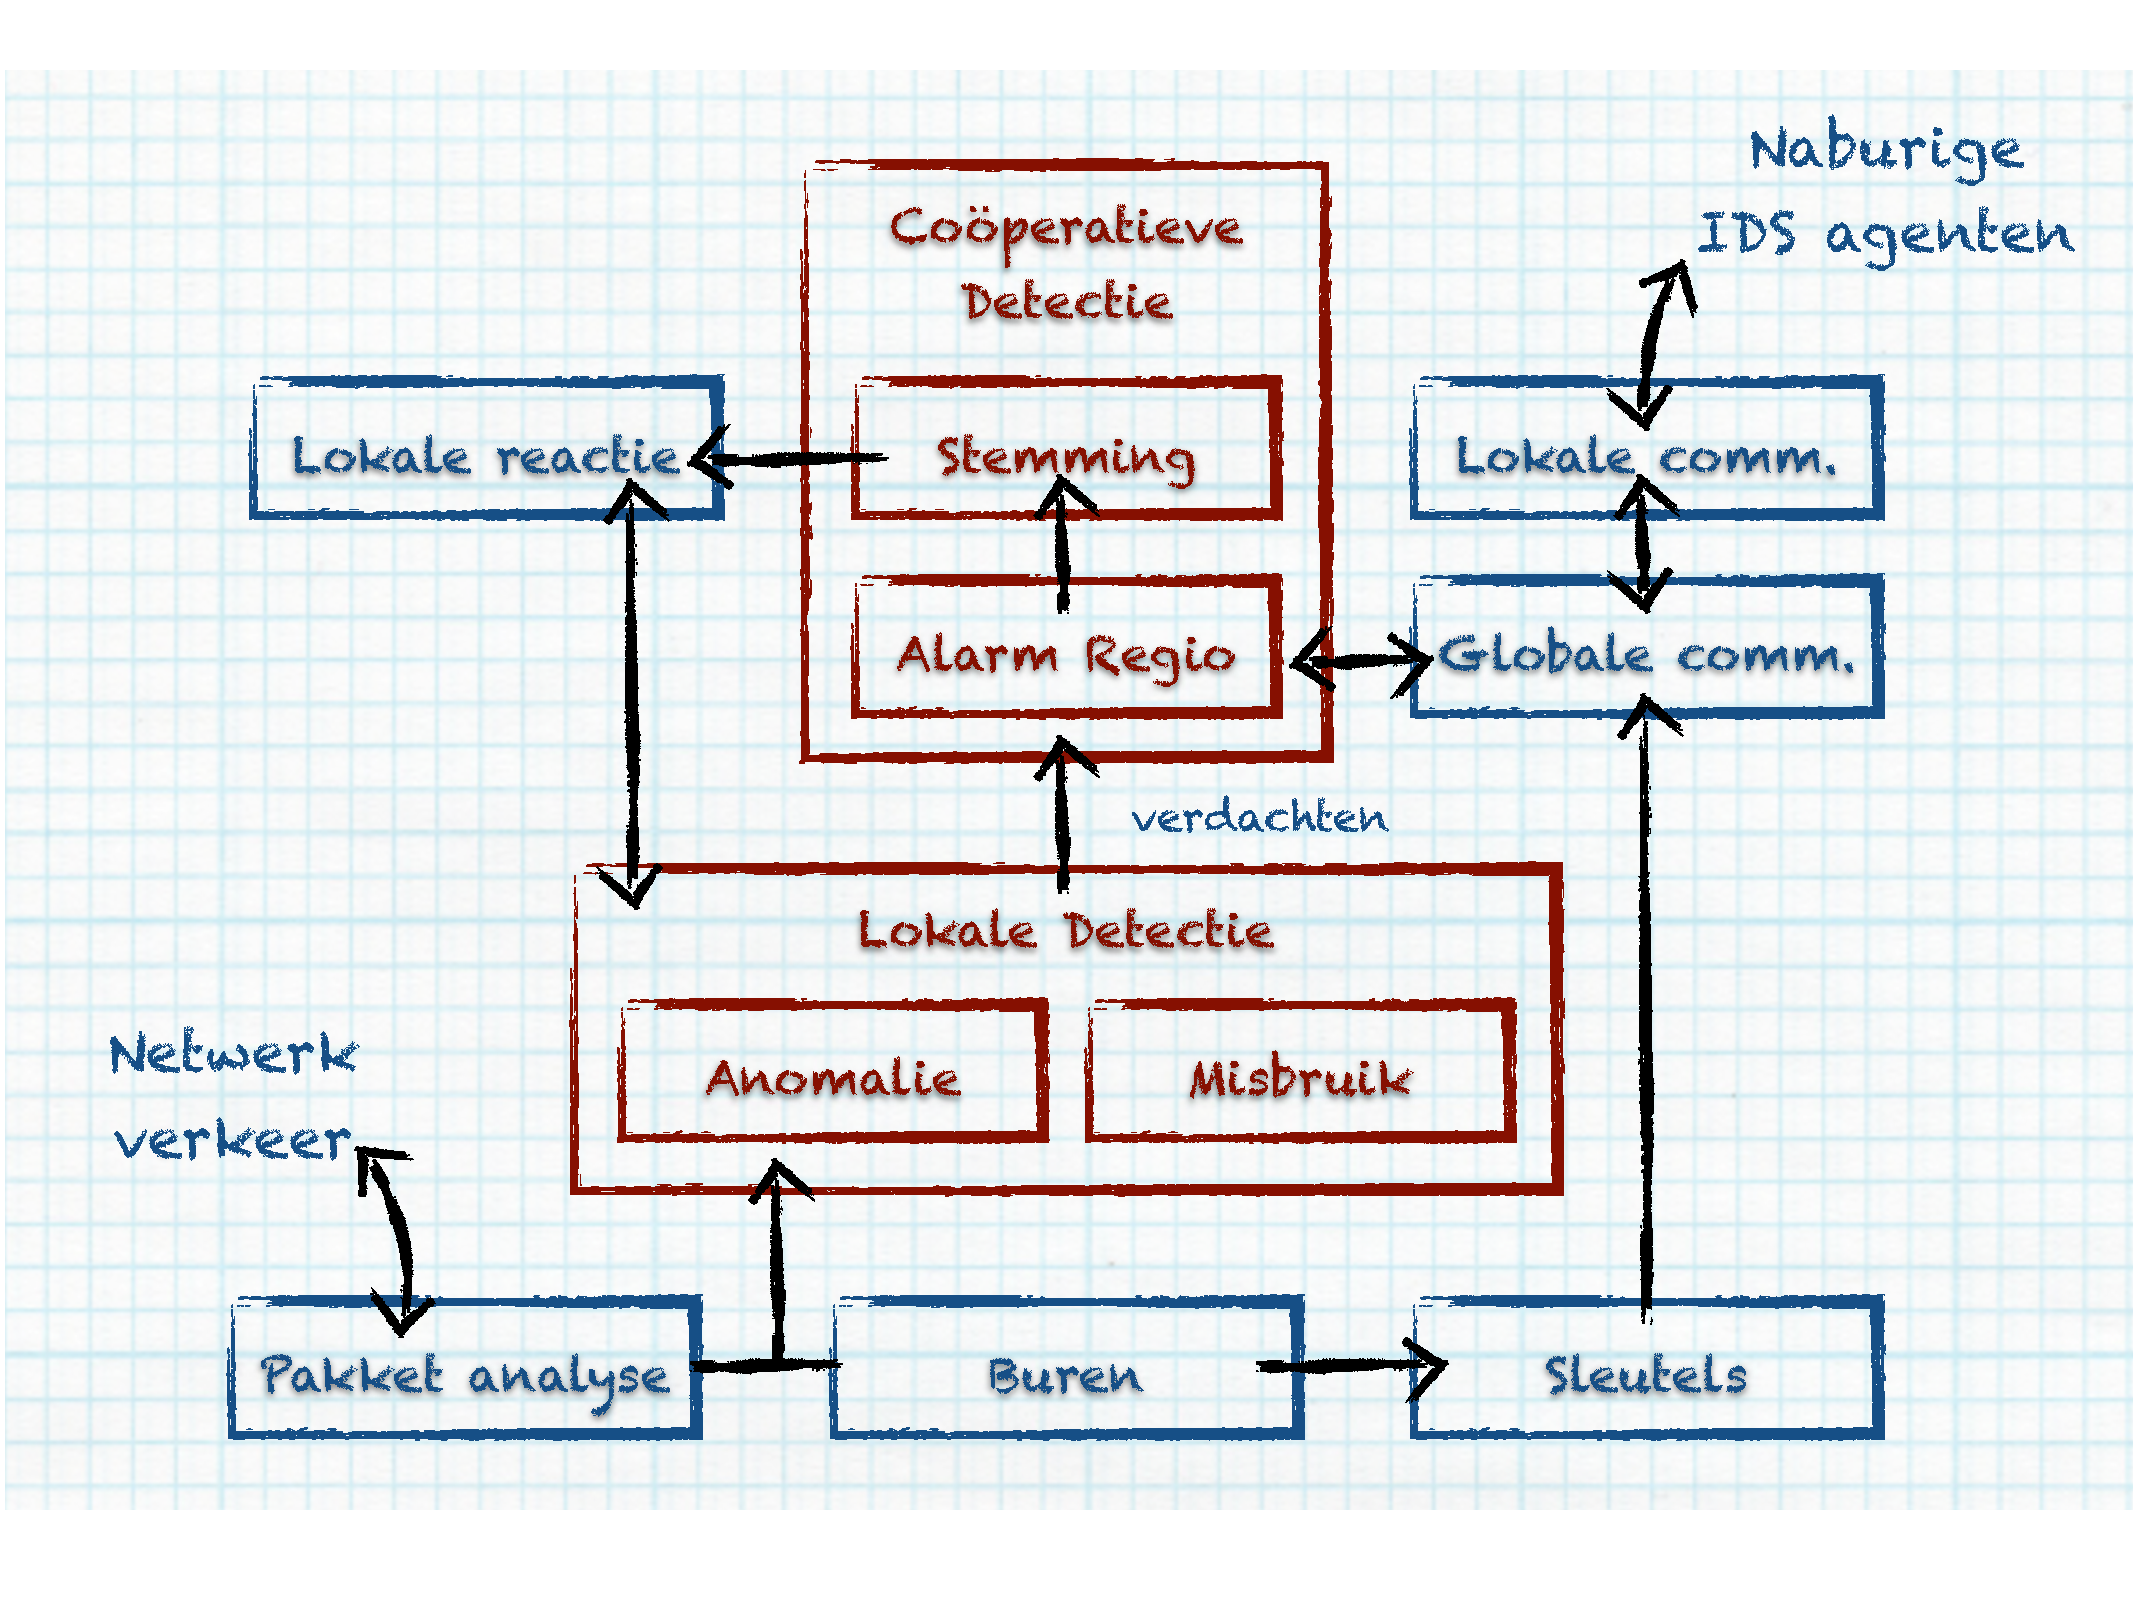
\includegraphics[width=0.9\linewidth]{resources/lidea-architecture.pdf}
  \caption[Architectuur van LIDeA]{Architectuur van LIDeA (Bron:\citep{krontiris2008lidea})}
  \label{fig:lidea-architecture}
\end{figure}


